% Relatorio tecnico -- Poco 861 (campo Lapa): integracao de dados e modelos preditivos
% Etapas 1, 1c, 1d, 1e, 1f (well_profile + ct_plugs + CLP-CSGM)
% Compilar: pdflatex poco861_etapa1_ml.tex (2x para referencias cruzadas)

\documentclass[11pt,a4paper]{article}

\usepackage[T1]{fontenc}
\usepackage[utf8]{inputenc}
\usepackage[brazil]{babel}
\usepackage{amsmath}
\usepackage{amssymb}
\usepackage{booktabs}
\usepackage{graphicx}
\graphicspath{%
  {figures/}%
  {../data/processed/ml_runs/diagnostics_861/figures/}%
  {../data/processed/ml_runs/well_profile/phi_lab/rf/}%
  {../data/processed/ml_runs/well_profile/phi_lab/compare/figures/}%
  {../data/processed/ml_runs/well_profile/phi_lab/alternatives/}%
  {../data/processed/ml_runs/well_profile/hfu/classifier/}%
  {../data/processed/ml_runs/ct_plugs/by_target/FZI_lab/wireline_only/}%
}
\usepackage{geometry}
\usepackage{hyperref}
\usepackage{caption}
\usepackage{subcaption}
\usepackage{siunitx}
\usepackage{float}

\geometry{margin=2.5cm}
\hypersetup{colorlinks=true, linkcolor=blue, citecolor=blue, urlcolor=blue}

% Notacao petrofisica (evita estilo de codigo no texto)
\newcommand{\philab}{\ensuremath{\phi_{\mathrm{lab}}}}
\newcommand{\fzilab}{\ensuremath{\mathrm{FZI}_{\mathrm{lab}}}}
\newcommand{\klab}{\ensuremath{k_{\mathrm{lab}}}}
\newcommand{\phiND}{\ensuremath{\phi_{\mathrm{ND}}}}
\newcommand{\phiN}{\ensuremath{\phi_{\mathrm{N}}}}
\newcommand{\phiS}{\ensuremath{\phi_{\mathrm{S}}}}
\newcommand{\deltaphi}{\ensuremath{\delta_{\phi}}}
\newcommand{\zvec}{\ensuremath{\mathbf{z}}}
\newcommand{\zzero}{\ensuremath{\mathbf{z}_0}}

\title{%
  Integração de dados e modelos preditivos no poço~861 (campo Lapa):\\
  perfil completo e plugs com microtomografia
}
\author{Grupo de Pesquisa cs-regressor}
\date{Junho de 2026}

\begin{document}

\maketitle

\begin{abstract}
Este relatorio descreve a Etapa~1 do projeto \emph{methods\_comparison} como
\textbf{diagnóstico local} no poço~861 (campo Lapa): intervalo 5205,91--5233,72~m,
87 amostras perfil+laboratório e dez plugs com microtomografia (microCT).
O objetivo foi verificar, \emph{antes} da modelagem física de velocidades,
quais propriedades petrofísicas os perfis convencionais conseguem prever com
validação espacialmente honesta.

Foram testados dois cenários: (i)~\textbf{perfil completo}---predição
ao longo de todo o intervalo perfurado, com validação por blocos
contíguos de profundidade; e (ii)~\textbf{plugs com microCT}---predição
plug a plug, deixando um plug de fora a cada rodada de teste.

Os principais resultados são: a porosidade medida em laboratório
(\philab) é a única propriedade com coeficiente de
determinação $R^2$ positivo e moderado ($R^2 \approx 0{,}15$) quando
prevista apenas com perfis; a previsão direta do indicador de zona de
fluxo (\fzilab) falha ($R^2 \approx -0{,}82$).
Um teste de referência (\emph{oracle}), que usa porosidade e
permeabilidade de laboratório como entrada, mostra que o FZI \emph{pode}
ser previsto quando essas informações estão disponíveis---o que
indica limite de informação nas curvas de perfil, e não falha
metodológica.

Complementarmente, testou-se reconstrução de curva de \philab{} por
CLP-CSGM com laboratório esparso nos dez plugs: a variante clássica com
prior de floresta aleatória (RF) no espaço latente não superou o RF
pontual ($\Delta\mathrm{RMSE} \approx +0{,}005$~pu); a variante
\emph{residual} ($\widehat{\phi}=\phi_{\mathrm{RF}}+\delta$) quase empata
com o RF ($\Delta\mathrm{RMSE} \approx +0{,}0003$~pu) e vence no bloco
superior.

Recomenda-se seguir para a Etapa~2 com modelos de meio efetivo (DEM/SC)
calibrados por unidade hidrodinâmica de fluxo (HFU), em vez de investir
em ajuste fino de algoritmos de aprendizado de máquina sobre perfis
isolados.
\end{abstract}

\section{Introdução}
\label{sec:intro}

\subsection{Contexto do poço e do projeto}

O poço~861 foi caracterizado em três escalas: curvas de perfil
registradas na perfuração, propriedades medidas em testemunhos de
laboratório (porosidade, permeabilidade, FZI) e morfologia dos poros
obtida por microCT em plugs de rocha.

O projeto \emph{methods\_comparison} busca, em etapas posteriores, estimar
as velocidades sísmicas de compressão ($V_p$) e cisalhamento ($V_s$)
por meio de modelos de meio efetivo---Differential Effective Medium (DEM)
e Self-Consistent (SC), implementados no Pyrockphys---calibrados por HFU.
Nesta fase \emph{não} tentamos prever $V_p$ ou $V_s$ diretamente; o foco
é responder: \emph{o que os perfis conseguem prever de forma confiável
antes de entrarmos na modelagem física?}

\subsection{Propriedades avaliadas}

\begin{itemize}
  \item \philab: porosidade total medida em laboratório (pu).
  \item \fzilab: Flow Zone Indicator, indicador de qualidade de
        zona de fluxo derivado de porosidade e permeabilidade de laboratório.
  \item \klab: permeabilidade absoluta medida em laboratório (mD).
  \item HFU: Hydraulic Flow Unit, unidade hidrodinâmica de fluxo
        (classes 1 a 4 neste poço).
\end{itemize}

\subsection{Organização do relatorio}

A Seção~\ref{sec:dados} apresenta os dados integrados.
A Seção~\ref{sec:protocolo} explica como os modelos foram testados.
As Seções~\ref{sec:diagnostico}--\ref{sec:alternativas} trazem os
resultados do perfil e dos plugs.
A Seção~\ref{sec:clp} documenta o CLP-CSGM com laboratório esparso
(Etapa~1f), incluindo o balanço dos termos do custo inverso, o papel
de $m$, a limitação de fidelidade visual (Seção~\ref{sec:clp_fidelity})
e o estudo de sensibilidade (Seção~\ref{sec:clp_sensitivity}).
A Seção~\ref{sec:discussao} interpreta os achados e a
Seção~\ref{sec:conclusoes} resume as recomendações.

\section{Dados e integração (Etapa~1)}
\label{sec:dados}

\subsection{Fontes e produtos}

Um fluxo automatizado de integração unificou perfis, resultados
de laboratório e descritores de microCT em dois conjuntos analíticos
(Tabela~\ref{tab:dataset}).

\begin{table}[H]
  \centering
  \caption{Conjuntos de dados integrados do poço~861.}
  \label{tab:dataset}
  \begin{tabular}{llrr}
    \toprule
    Conjunto & Uso & Amostras & Profundidade (m) \\
    \midrule
    Perfil enriquecido com laboratório
      & Perfil ao longo do poço & 87 & 5205,91--5233,72 \\
    Plugs integrados com microCT
      & Amostras plug a plug & 10 & plugs + perfil adjacente \\
    \bottomrule
  \end{tabular}
\end{table}

Na Tabela~\ref{tab:dataset}, o conjunto de 87 amostras cobre quase 28~m de coluna perfurada e é a
base principal para avaliar se os perfis preveem propriedades de
laboratório ao longo do poço.
Os dez plugs com microCT representam uma amostragem muito menor e mais
cara: servem para calibrar propriedades de textura e geometria de poros,
não para substituir o perfil completo.
A sobreposição de apenas oito profundidades com CT indica que a
maioria das amostras de perfil não possui imagem tridimensional
associada---o microCT complementa, mas não cobre todo o intervalo.

No conjunto de 87 amostras, oito profundidades possuem plug de microCT
associado.
A consistência entre profundidades de plugs e perfis foi verificada por
controle de qualidade da integração.

\subsection{Variáveis de entrada e de saída}

As curvas de perfil usadas como \emph{entrada} dos modelos estão na
Tabela~\ref{tab:features}.
As \emph{saídas} testadas foram \philab, \fzilab, \klab{} e HFU.

Importante: ao prever FZI, não podemos usar no modelo variáveis que
já carregam a mesma informação do alvo (por exemplo, porosidade e
permeabilidade de laboratório, que entram no cálculo do FZI).
Essa regra---detalhada na Seção~\ref{sec:protocolo}---evita que o
modelo ``cola'' no resultado de laboratório em vez de aprender do perfil.

\begin{table}[H]
  \centering
  \caption{Curvas de perfil usadas como entrada
           (perfil completo e plugs com microCT, somente perfil).}
  \label{tab:features}
  \begin{tabular}{ll}
    \toprule
    Curva & Significado \\
    \midrule
    GR (API) & Gama raio \\
    $\rho_b$ (g/cc) & Densidade \\
    $R_t$ profunda e rasa & Resistividade \\
    $\phi_{\mathrm{N}}$, $\phi_{\mathrm{S}}$, $\phi_{\mathrm{ND}}$ (pu)
      & Porosidades estimadas pelo perfil \\
    Litotipo & Código 1--4 (Tabela~\ref{tab:lithotypes}) \\
    \bottomrule
  \end{tabular}
\end{table}

A Tabela~\ref{tab:features} lista as oito curvas de perfil que um petrofísico usaria em
uma interpretação convencional: litologia (GR, litotipo), porosidade
(neutrón, sónica, densidade-neutrón) e fluido/rocha (resistividade).
Não incluímos curvas derivadas de laboratório no conjunto de entrada,
para que o modelo seja avaliado de forma justa: ele deve aprender apenas
do que estaria disponível \emph{antes} da análise de testemunho.
No cenário com microCT, os descritores de imagem acrescentam informação
de morfologia de poros que o perfil não resolve---por exemplo, forma e
conectividade dos poros.

No cenário com perfil acrescido de descritores de microCT, acrescentam-se
sete variáveis derivadas da imagem (porosidade da imagem, razão de
aspecto dos poros, fração de sólidos corrigida, entre outros).

\subsection{Distribuição de HFU}

As classes de HFU não estão igualmente representadas:
HFU1 ($n=42$), HFU2 ($n=29$), HFU3 ($n=10$), HFU4 ($n=6$).
Esse desbalanceamento exige cautela na interpretação da acurácia
dos classificadores (Seção~\ref{sec:alternativas}).
Em termos práticos, um modelo que sempre prediz HFU1 acertaria
$42/87 \approx 48\%$ das amostras sem aprender padrão algum do perfil.
Por isso, além da acurácia global, reportamos acurácia balanceada e
F1 macro, que penalizam o desempenho nas classes minoritárias (HFU3 e HFU4).

\subsection{Litotipos e classes HFU codificados}

O poço~861 situa-se no \textbf{campo Lapa} (carbonatos pré-sal, Bacia de Santos);
não confundir o nome do campo com o código de \texttt{Lithotype}.
As fácies interpretadas em testemunho seguem a aba \texttt{Legend} de
\texttt{Auddys\_table.xlsx} (Tabela~\ref{tab:lithotypes}).
A coluna \texttt{HFU} usa a mesma convenção da planilha
(Tabela~\ref{tab:hfu_legend}).

\begin{table}[H]
  \centering
  \caption{Codificação de litotipos no perfil enriquecido ($n=87$).}
  \label{tab:lithotypes}
  \begin{tabular}{clr}
    \toprule
    Código & Nome (Legend) & Amostras \\
    \midrule
    1 & Grainstone & 25 \\
    2 & Shrubs & 42 \\
    3 & Laminite & 7 \\
    4 & Spherulite & 13 \\
    \bottomrule
  \end{tabular}
\end{table}

\begin{table}[H]
  \centering
  \caption{Codificação de HFU (Hydrocarbon Flow Unit) no mesmo dataset.}
  \label{tab:hfu_legend}
  \begin{tabular}{clr}
    \toprule
    Código & Classe (Legend) & Amostras \\
    \midrule
    1 & Poor & 42 \\
    2 & Medium & 29 \\
    3 & Good & 10 \\
    4 & Excellent & 6 \\
    \bottomrule
  \end{tabular}
\end{table}

Na Tabela~\ref{tab:lithotypes}, \emph{Shrubs} e \emph{Spherulite} são os
litotipos mais frequentes no intervalo; \emph{Grainstone} concentra-se no
bloco central de validação (Tabela~\ref{tab:depthblocks}).
A variável \texttt{Lithotype} entra como feature categórica nos modelos de
perfil (junto com GR e demais curvas wireline).

\section{Protocolo de avaliação}
\label{sec:protocolo}

\subsection{Evitar uso indevido de variáveis de laboratório}

Para cada propriedade alvo, excluímos do conjunto de entrada ($X$) as
colunas que repetiria informação já presente no alvo ($y$).
A Tabela~\ref{tab:leakage} resume essas exclusões.

\begin{table}[H]
  \centering
  \caption{Variáveis de laboratório excluídas da entrada, por alvo.}
  \label{tab:leakage}
  \begin{tabular}{ll}
    \toprule
    Alvo & Não usar como entrada \\
    \midrule
    \philab & \philab, RQI, \fzilab \\
    \fzilab & \fzilab, \philab, \klab, RQI, HFU \\
    HFU & HFU, \fzilab, RQI \\
    \bottomrule
  \end{tabular}
\end{table}

Na Tabela~\ref{tab:leakage}, ao prever FZI, por exemplo, excluímos \philab{} e \klab{}
porque o FZI é calculado a partir dessas duas grandezas---usá-las como
entrada faria o modelo ``copiar'' o resultado de laboratório, gerando
$R^2$ artificialmente alto que não refletiria o poder preditivo real do
perfil.
A mesma lógica vale para RQI e HFU, que carregam informação
redundante com FZI e permeabilidade.

\subsection{Validação no perfil completo}

Dividimos as 87 amostras em \textbf{três blocos contíguos de
profundidade} (cerca de 29 amostras cada).
Em cada rodada de validação (\emph{fold}), dois blocos servem para
treinar o modelo e o terceiro, reservado, serve para testar.
Esse esquema---chamado \emph{validação cruzada por blocos de
profundidade}---simula a situação real de prever um intervalo que o
modelo ainda não viu, sem misturar profundidades vizinhas entre treino e
teste.

Cada amostra recebe uma predição \emph{out-of-fold} (OOF): ela só entra
no teste quando o seu bloco de profundidade está reservado, de modo que
o modelo não viu aquela faixa no treino.
As métricas e figuras de \philab{} nesta seção usam esse protocolo.

Isso contrasta com a divisão aleatória 80\%/20\%, que costuma
\emph{superestimar} o desempenho em dados de poço, pois amostras
próximas em profundidade (e geologicamente semelhantes) acabam tanto no
treino quanto no teste.

A Tabela~\ref{tab:depthblocks} mostra que os três blocos são
petrofísicamente distintos: o bloco central concentra \emph{Grainstone}
(litotipo~1) e a HFU1; o bloco inferior apresenta maior permeabilidade
média e litotipos \emph{Shrubs}, \emph{Laminite} e \emph{Spherulite}.

\begin{table}[H]
  \centering
  \caption{Características médias de cada bloco de profundidade usado
           na validação ($n \approx 29$ amostras por bloco).
           Contagens de litotipo seguem a Tabela~\ref{tab:lithotypes}.}
  \label{tab:depthblocks}
  \scriptsize
  \begin{tabular}{ccrrrrrrrrr}
    \toprule
    Bloco & Prof.\ (m) & $\overline{\mathrm{FZI}}$ & $\overline{\phi_{\mathrm{lab}}}$
      & $\overline{k_{\mathrm{lab}}}$ & HFU1 & HFU2
      & Grain. & Shrubs & Lamin. & Spher. \\
    & & & (pu) & (mD) & & & (1) & (2) & (3) & (4) \\
    \midrule
    0 & 5206--5214 & 1,39 & 0,092 & 3,6  & 16 & 8  & 6  & 19 & 3 & 1 \\
    1 & 5215--5223 & 1,25 & 0,115 & 9,5  & 19 & 7  & 19 & 10 & 0 & 0 \\
    2 & 5225--5234 & 1,87 & 0,145 & 54,6 & 7  & 14 & 0  & 13 & 4 & 12 \\
    \bottomrule
  \end{tabular}
\end{table}

Em detalhe, o bloco~0 (5206--5214~m) é o mais ``tight'': porosidade média de
0,092~pu e permeabilidade média de apenas 3,6~mD.
O bloco~1 (5215--5223~m) concentra 19 das 29 amostras de \emph{Grainstone}
(litotipo~1) e é onde o modelo de FZI apresenta pior desempenho
(Tabela~\ref{tab:fzi_folds})---o perfil não distingue bem as variações
de textura nesse intervalo homogêneo em litologia.
O bloco~2 (5225--5234~m) é o mais ``permeável'': $\overline{k_{\mathrm{lab}}}
= 54{,}6$~mD e $\overline{\phi_{\mathrm{lab}}} = 0{,}145$~pu, sem
\emph{Grainstone} (litotipo~1); predominam \emph{Shrubs} e \emph{Spherulite};
é também onde o RF de porosidade perde desempenho ($R^2 = -0{,}157$),
sugerindo que a relação perfil--laboratório muda nesse subintervalo.

\subsection{Validação nos plugs com microCT}

Com apenas 10 plugs, usamos validação \emph{leave-one-plug-out}
(LOPO): em cada uma das dez rodadas, nove plugs treinam e um plug
específico) testa.
O $R^2$ reportado é calculado sobre as dez predições feitas fora
da amostra de treino (predições OOF, \emph{out-of-fold}).

\subsection{Modelos testados}

Na Etapa~1c compararam-se cinco regressores: Random Forest (RF), Gradient
Boosting, XGBoost, rede neural (MLP) e regressão linear.
Na Etapa~1d/1e: RF para \philab{}; Ridge e GAM como alternativas
para porosidade; e regressão logística e RF balanceado para
classificar HFU.

Não houve busca automática de hiperparâmetros nesta fase.
O RF de produção usa 200 árvores de decisão e semente fixa para
reprodutibilidade.

\subsection{Como ler o $R^2$}

O coeficiente de determinação $R^2$ mede o quanto o modelo explica a
variação do alvo em relação a simplesmente prever a média.
Valores próximos de 1 indicam bom ajuste; valores próximos de 0 indicam
desempenho semelhante à média; valores \textbf{negativos} significam
que o modelo erra \emph{mais} do que usar apenas a média do treino---um
sinal claro de falha preditiva.

\section{Diagnóstico: o que os perfis conseguem explicar? (Etapa~1c)}
\label{sec:diagnostico}

Antes de treinar modelos complexos, analisamos a correlação linear
(Pearson) entre cada curva de perfil e cada propriedade alvo.
Correlação alta sugere que a curva carrega informação útil;
correlação baixa indica que o perfil, sozinho, dificilmente
conseguirá prever aquela propriedade.

\subsection{Correlação perfil--FZI}

A Figura~\ref{fig:fzi_corr} mostra as correlações entre curvas de
perfil e \fzilab{}.
A melhor curva de perfil (\phiND{}) atinge apenas $r \approx 0{,}31$;
gama raio e resistividade são praticamente nulas.

Em contraste, variáveis de laboratório---que não entram no modelo por
serem derivadas do próprio FZI---correlacionam fortemente
(Tabela~\ref{tab:corr_fzi}).
Isso explica por que o FZI é difícil de prever só com perfis: o
sinal relevante está nas medidas de laboratório, não nas curvas.

\begin{figure}[H]
  \centering
  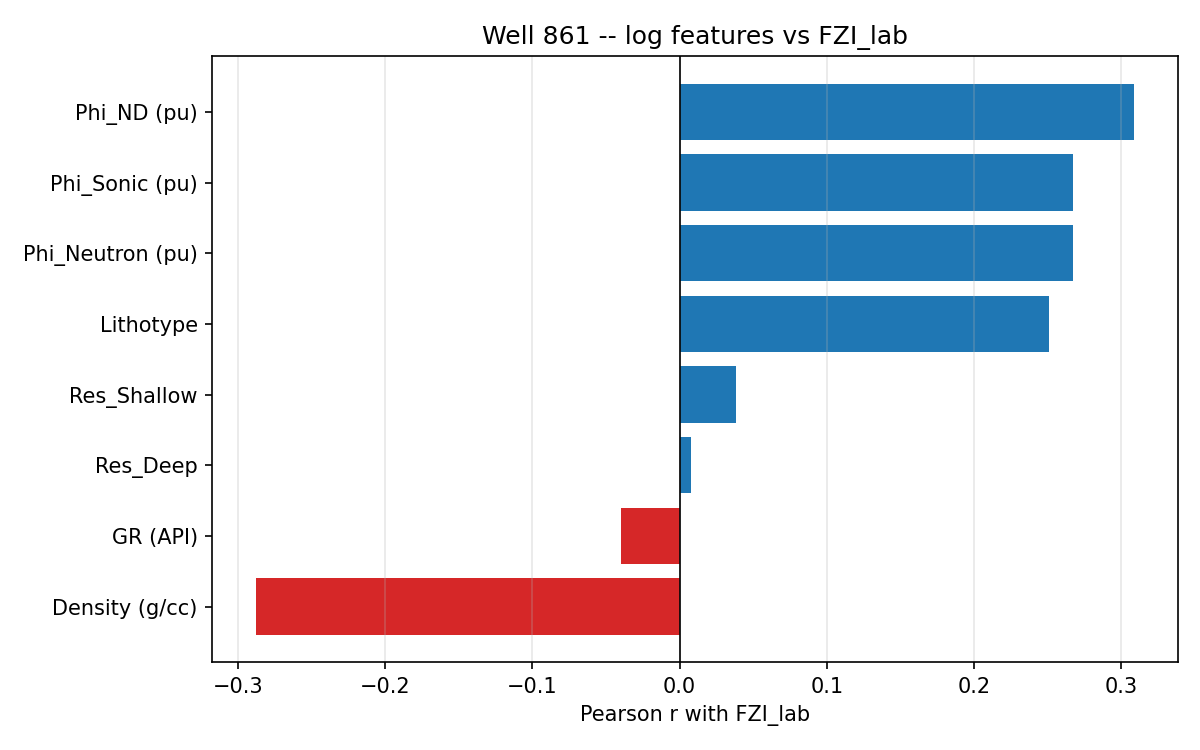
\includegraphics[width=0.85\linewidth]{figures/fig_fzi_log_correlations}
  \caption{Correlação de Pearson entre curvas de perfil e
           \fzilab{} ($n=87$). Barras curtas indicam pouca
           relação linear.}
  \label{fig:fzi_corr}
\end{figure}

A Figura~\ref{fig:fzi_corr} confirma visualmente que todas as barras de correlação com curvas de perfil são
curtas em comparação ao que seria necessário para uma predição
confiável de FZI.
A melhor curva (\phiND{}, $r \approx 0{,}31$) explica menos de 10\%
da variância do FZI ($r^2 \approx 0{,}10$).
Gama raio e resistividade praticamente não se relacionam com FZI neste
intervalo---o que faz sentido geologicamente, pois FZI depende da geometria
e conectividade dos poros (textura), não apenas da litologia ou do
conteúdo de fluido detectado pelo perfil.

\begin{table}[H]
  \centering
  \caption{Correlação de Pearson com \fzilab{}: laboratório
           versus perfil.}
  \label{tab:corr_fzi}
  \begin{tabular}{lrr}
    \toprule
    Variável & $r$ & $|r|$ \\
    \midrule
    RQI (laboratório; excluída do modelo) & 0,887 & 0,887 \\
    $k_{\mathrm{lab}}$ (excluída) & 0,709 & 0,709 \\
    HFU (excluída para FZI) & 0,614 & 0,614 \\
    Phi\_ND (perfil) & 0,308 & 0,308 \\
    GR (perfil) & $-0{,}040$ & 0,040 \\
    \bottomrule
  \end{tabular}
\end{table}

Na Tabela~\ref{tab:corr_fzi}, o contraste entre laboratório e perfil é marcante.
RQI (Quality Index) correlaciona com FZI em $r = 0{,}89$ porque ambos
descrevem a mesma qualidade de zona de fluxo; permeabilidade ($r = 0{,}71$)
e HFU ($r = 0{,}61$) também carregam essa informação.
Já a melhor curva de perfil (\phiND{}) atinge apenas $r = 0{,}31$---
cerca de três vezes menor que RQI.
Isso antecipa o resultado regressivo: sem permeabilidade e textura de
laboratório, o perfil não tem base suficiente para prever FZI.

\subsection{Correlação perfil--porosidade}

Para \philab{}, as porosidades de perfil são bem mais
informativas (Tabela~\ref{tab:corr_phi}), o que é consistente com o
melhor desempenho regressivo observado adiante
(Seção~\ref{sec:wellprofile}).

\begin{table}[H]
  \centering
  \caption{Correlação de Pearson com \philab{} (pu).}
  \label{tab:corr_phi}
  \begin{tabular}{lr}
    \toprule
    Variável & $r$ \\
    \midrule
    Phi\_Neutron (perfil) & 0,737 \\
    Phi\_ND (perfil) & 0,701 \\
    Density (perfil) & $-0{,}670$ \\
    Phi\_Sonic (perfil) & 0,667 \\
    \bottomrule
  \end{tabular}
\end{table}

Para porosidade, a Tabela~\ref{tab:corr_phi} mostra situação oposta à do FZI:
As três porosidades de perfil (\phiN{}, \phiND{},
\phiS{}) correlacionam entre 0,67 e 0,74 com \philab{}---
valores considerados fortes em petrofísica de carbonatos.
A densidade apresenta correlação negativa ($r = -0{,}67$), coerente com
o fato de que rocha mais densa tende a ser menos porosa.
Esse alinhamento entre correlação e desempenho regressivo confirma que
porosidade é a propriedade mais natural de se estimar a partir de perfis
neste poço.

\subsection{Teste de referência (\emph{oracle})}

Para distinguir ``falta de informação no perfil'' de ``modelo mal
escolhido'', rodamos um experimento de referência: o RF recebe
\philab{} e \klab{} como entrada para prever FZI.
Esse teste \emph{oracle} não é aplicável em produção (usa
dados de laboratório que não teríamos antes da análise), mas serve
para diagnóstico.

A Figura~\ref{fig:oracle} compara o desempenho bloco a bloco.
Com perfis isolados, o modelo falha no bloco~1 ($R^2 \approx -1{,}95$).
Com o teste \emph{oracle}, o $R^2$ sobe para valores entre 0,37 e 0,88 nos
blocos 0 e 1, com média global de aproximadamente 0,69.
Confirmamos que o FZI \emph{tem} sinal previsível---mas esse sinal vem
de porosidade e permeabilidade de laboratório, não das curvas de perfil.

\begin{figure}[H]
  \centering
  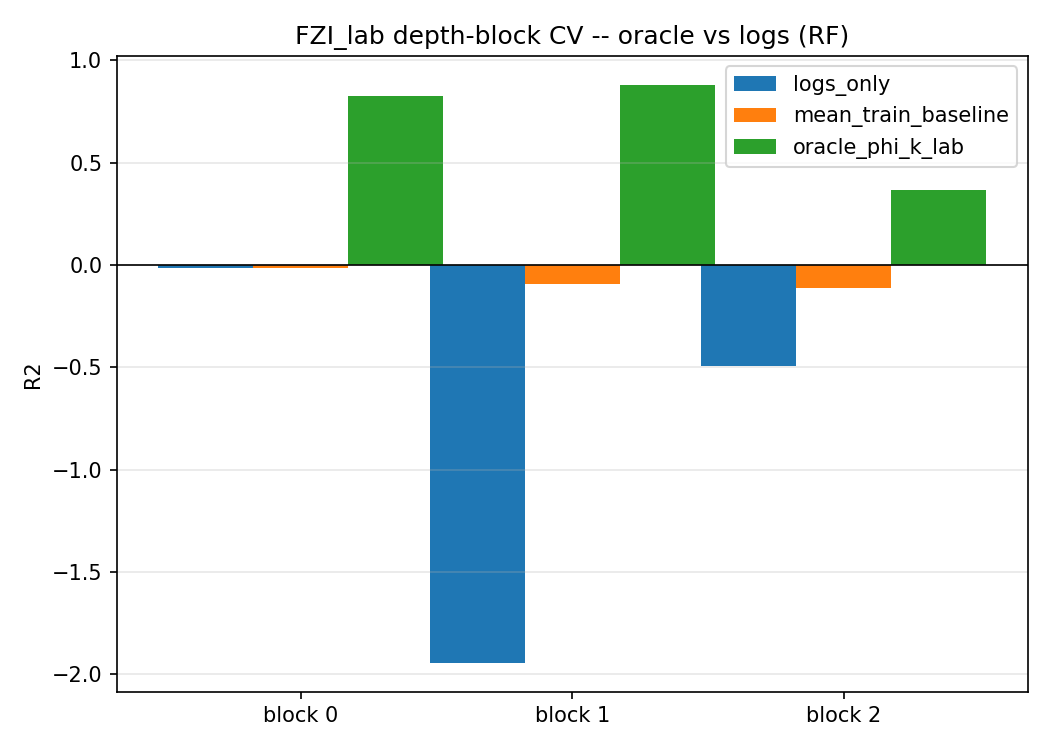
\includegraphics[width=0.78\linewidth]{figures/fig_fzi_oracle_vs_logs}
  \caption{$R^2$ por bloco de profundidade para \fzilab{}:
           apenas perfis versus teste \emph{oracle}
           (\philab{} + \klab{} de laboratório).}
  \label{fig:oracle}
\end{figure}

A Figura~\ref{fig:oracle} ilustra dois cenários lado a lado para cada bloco de profundidade.
Com perfis isolados (barras negativas no bloco~1), o modelo não consegue
capturar a variação de FZI---o $R^2$ de $-1{,}95$ significa que as
predições são piores do que simplesmente usar a média do treino.
Com o teste \emph{oracle} (porosidade e permeabilidade de laboratório como
entrada), o $R^2$ sobe para valores entre 0,37 e 0,88, com média global de
aproximadamente 0,69.
A lição é direta: o FZI \emph{contém} informação previsível,
mas essa informação reside em propriedades medidas em laboratório,
não nas curvas de perfil disponíveis.
O problema não é o algoritmo (Random Forest), e sim o que o perfil consegue
``ver'' da textura do meio poroso.

\section{Resultados no perfil completo}
\label{sec:wellprofile}

\subsection{Comparação entre propriedades alvo}

A Tabela~\ref{tab:targets_rf} resume o Random Forest para três alvos.
Apenas \philab{} apresenta $R^2$ médio positivo.
A Figura~\ref{fig:target_r2} compara cada alvo com a referência de
prever simplesmente a média do treino.

\begin{table}[H]
  \centering
  \caption{Random Forest no perfil completo (validação por blocos de
           profundidade, $n=87$). RMSE: erro quadrático médio.}
  \label{tab:targets_rf}
  \begin{tabular}{lrrr}
    \toprule
    Alvo & RMSE médio & $R^2$ médio & Desvio do $R^2$ \\
    \midrule
    Phi\_lab (pu) & 0,033 & \textbf{0,146} & 0,222 \\
    FZI\_lab & 1,813 & $-0{,}819$ & 0,820 \\
    $k_{\mathrm{lab}}$ (mD) & 76,2 & $-15{,}4$ & 18,4 \\
    \bottomrule
  \end{tabular}
\end{table}

\begin{figure}[H]
  \centering
  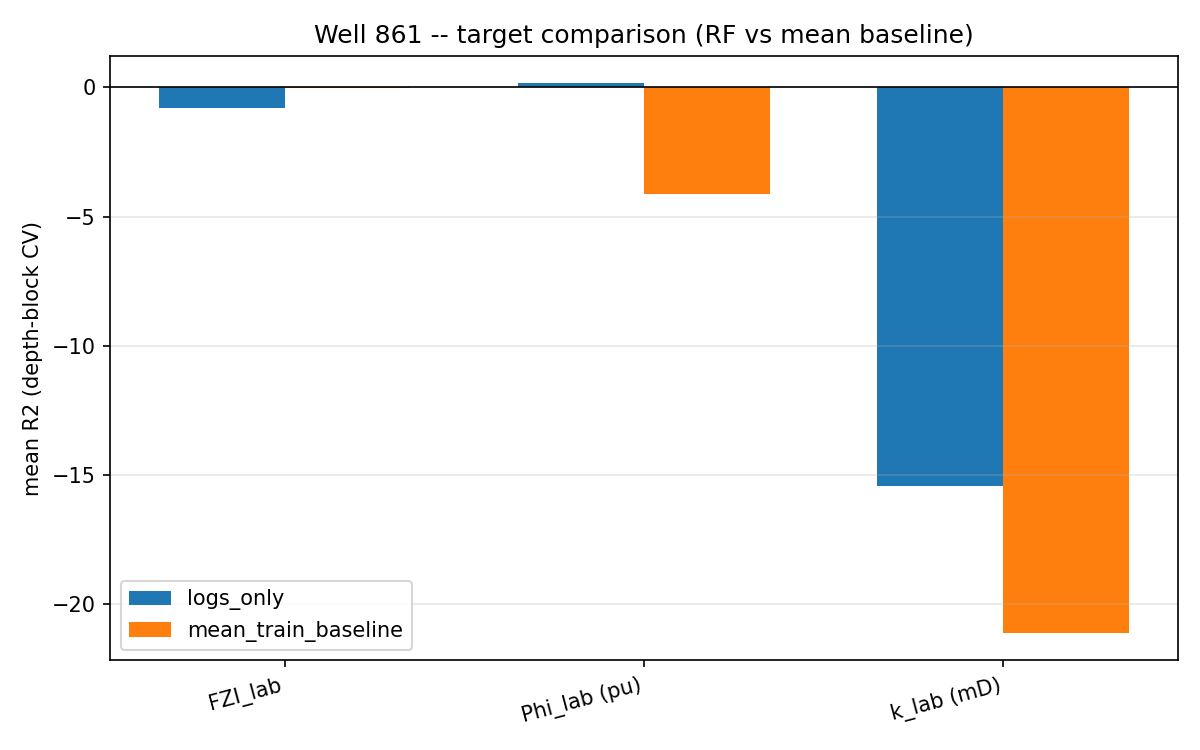
\includegraphics[width=0.82\linewidth]{figures/fig_target_comparison_r2}
  \caption{$R^2$ médio (RF, validação por blocos) para cada alvo,
           comparado à referência de prever a média.}
  \label{fig:target_r2}
\end{figure}

Em conjunto, apenas porosidade supera a referência de prever a média; FZI e permeabilidade permanecem com $R^2$ negativo.

\emph{Porosidade} ($R^2 = 0{,}146$, RMSE $= 0{,}033$~pu): o modelo explica
cerca de 15\% da variância de \philab{}, com erro típico de
0,033 porosidade absoluta (3,3 pontos percentuais).
Para um intervalo com porosidade entre $\sim$0,07 e 0,20~pu, isso representa
um erro relativo moderado---utilizável como insumo preliminar para DEM/SC,
mas não como substituto da medição de laboratório.
O desvio padrão do $R^2$ (0,222) indica que o desempenho varia bastante
entre blocos (confirmado na Tabela~\ref{tab:phi_folds}).

\emph{FZI} ($R^2 = -0{,}819$, RMSE $= 1{,}813$): resultado claramente
inaceitável.
Um $R^2$ negativo próximo de $-1$ significa que o modelo duplica o erro
em relação a prever a média.
Na Figura~\ref{fig:target_r2}, a barra de FZI fica muito abaixo da linha de
referência (média), confirmando a falha.

\emph{Permeabilidade} ($R^2 = -15{,}4$, RMSE $= 76$~mD): o pior resultado.
Permeabilidade em carbonatos costuma ter distribuição com cauda longa
(valores que vão de menos de 1~mD a centenas de mD), o que dificulta
qualquer regressão com apenas 87 amostras e oito curvas de perfil.
O RMSE de 76~mD parece alto, mas reflete a enorme variância de $k_{\mathrm{lab}}$
no bloco~2 ($\overline{k} = 54{,}6$~mD com valores individuais muito maiores).

\subsection{O algoritmo importa?}

A Tabela~\ref{tab:regressors} compara cinco algoritmos sob o mesmo
protocolo, com colunas correspondentes a \emph{alvos diferentes}.
Para isolar o efeito do algoritmo em porosidade, a
Tabela~\ref{tab:regressors_phi} resume apenas \philab{} ($n=87$,
predições OOF em três blocos).
Para FZI e permeabilidade em Tabela~\ref{tab:regressors}, \emph{todos}
falham.
Isso reforça que o problema não está no tipo de algoritmo, e sim
na quantidade de informação disponível nas curvas de perfil.

\begin{table}[H]
  \centering
  \caption{Cinco regressores para \philab{} (perfil completo,
           predições OOF, três blocos de profundidade).}
  \label{tab:regressors_phi}
  \begin{tabular}{lrr}
    \toprule
    Algoritmo & RMSE OOF (pu) & $R^2$ OOF médio \\
    \midrule
    Random Forest & 0,033 & \textbf{0,146} \\
    Regressão linear & 0,036 & $-0{,}261$ \\
    XGBoost & 0,036 & $-0{,}099$ \\
    Gradient Boosting & 0,040 & $-0{,}313$ \\
    Rede neural (MLP) & 0,097 & $-6{,}871$ \\
    \bottomrule
  \end{tabular}
\end{table}

\begin{table}[H]
  \centering
  \caption{Comparação de cinco regressores no perfil completo:
           $R^2$ OOF médio por alvo (cada coluna é um alvo distinto).}
  \label{tab:regressors}
  \small
  \begin{tabular}{lrrr}
    \toprule
    Algoritmo & \philab{} & \fzilab{} & $k_{\mathrm{lab}}$ \\
    \midrule
    Random Forest & \textbf{0,146} & $-0{,}819$ & $-15{,}4$ \\
    Rede neural (MLP) & $-6{,}871$ & $-0{,}251$ & $-0{,}026$ \\
    XGBoost & $-0{,}099$ & $-2{,}308$ & $-72{,}0$ \\
    Regressão linear & $-0{,}261$ & $-2{,}392$ & $-24{,}2$ \\
    Gradient Boosting & $-0{,}313$ & $-1{,}582$ & $-22{,}2$ \\
    \bottomrule
  \end{tabular}
\end{table}

Na Tabela~\ref{tab:regressors_phi}, o Random Forest é o único com $R^2$
positivo em \philab{}; os demais variam entre $-0{,}10$ (XGBoost) e
$-6{,}87$ (MLP).
O MLP, em particular, apresenta $R^2 = -6{,}87$---sinal de que a rede neural,
com poucos dados e sem ajuste de hiperparâmetros, não é adequada aqui.
Para FZI, todos os algoritmos falham, embora o MLP ($R^2 = -0{,}25$) pareça
``menos ruim'' que o RF---isso \emph{não} significa que MLP é melhor:
$R^2$ negativo próximo de zero ainda indica desempenho inaceitável, e a
diferença entre algoritmos é pequena frente ao limite informacional
identificado no diagnóstico (Seção~\ref{sec:diagnostico}).
Para permeabilidade, o MLP ($R^2 = -0{,}03$) também parece competitivo, mas
novamente todos os valores são negativos ou próximos de zero---nenhum
modelo é viável para prever $k_{\mathrm{lab}}$ a partir de perfis.

\subsection{Porosidade de laboratório: modelo principal}

O RF para \philab{} atinge RMSE médio de \SI{0.033}{pu} e
$R^2 = 0{,}146$ (Tabela~\ref{tab:phi_folds}).
O desempenho varia por bloco: os blocos 0 e 1 são positivos; o bloco 2
é negativo, coincidindo com o intervalo de maior permeabilidade média
(Tabela~\ref{tab:depthblocks}).

\begin{table}[H]
  \centering
  \caption{RF para \philab{}: resultado em cada bloco de teste.}
  \label{tab:phi_folds}
  \begin{tabular}{ccrrr}
    \toprule
    Bloco & Prof.\ teste (m) & RMSE & $R^2$ & Amostras de teste \\
    \midrule
    0 & 5206--5214 & 0,015 & 0,367 & 29 \\
    1 & 5215--5223 & 0,037 & 0,227 & 29 \\
    2 & 5225--5234 & 0,047 & $-0{,}157$ & 29 \\
    \midrule
    Média & -- & 0,033 & 0,146 & -- \\
    \bottomrule
  \end{tabular}
\end{table}

A Tabela~\ref{tab:phi_folds} revela \emph{onde} o modelo funciona e onde falha.

\emph{Bloco~0} (5206--5214~m): $R^2 = 0{,}367$, RMSE $= 0{,}015$~pu---o
melhor resultado.
Este intervalo tem menor porosidade e permeabilidade
(Tabela~\ref{tab:depthblocks}), e a relação entre porosidades de perfil
e \philab{} é mais estável.

\emph{Bloco~1} (5215--5223~m): $R^2 = 0{,}227$, RMSE $= 0{,}037$~pu---desempenho
positivo, porém mais fraco.
Predomina \emph{Grainstone} (litotipo~1); o erro aumenta porque a variabilidade de
\philab{} dentro do bloco é menor e mais difícil de capturar.

\emph{Bloco~2} (5225--5234~m): $R^2 = -0{,}157$, RMSE $= 0{,}047$~pu---o modelo
falha neste intervalo.
Aqui a permeabilidade média salta para 54,6~mD e a porosidade média para
0,145~pu, sem \emph{Grainstone} (litotipo~1).
O perfil parece responder de forma diferente neste subintervalo mais
permeável, e o modelo treinado nos outros blocos não generaliza.

Em resumo: o $R^2$ médio de 0,146 mascara desempenho heterogêneo---bom nos
dois blocos superiores, ruim no inferior.

As Figuras~\ref{fig:phi_oof_panels}--\ref{fig:phi_oof_rmse_fold} mostram
o desempenho \emph{ao longo da profundidade}, com o mesmo protocolo OOF
das tabelas: observado (tracejado) versus predito (colorido) para RF,
Gradient Boosting, MLP e regressão linear; linhas horizontais tracejadas
indicam os limites entre blocos de teste.
A Figura~\ref{fig:phi_oof_rmse_fold} quantifica o RMSE OOF por bloco:
RF e regressão linear lideram; MLP degrada fortemente no bloco~2.

\begin{figure}[H]
  \centering
  
\includegraphics[width=\linewidth]{phi_lab_oof_depth_panels.png}
  \caption{\philab{} ao longo da profundidade: observado (tracejado) e
           predições OOF por regressor (RF, Gradient Boosting, MLP e
           regressão linear). Mesmo protocolo da Tabela~\ref{tab:phi_folds}
           ($n=87$, oito curvas wireline, três blocos).}
  \label{fig:phi_oof_panels}
\end{figure}

\begin{figure}[H]
  \centering
  
\includegraphics[width=0.78\linewidth]{phi_lab_oof_rmse_by_depth_fold.png}
  \caption{RMSE OOF por bloco de profundidade para \philab{} (RF, GB, MLP
           e LR). O erro cresce no bloco~2 em todos os algoritmos.}
  \label{fig:phi_oof_rmse_fold}
\end{figure}

\emph{RF (verde):} acompanha \philab{} nos blocos~0--1 e desvia no
bloco profundo.
\emph{Regressão linear (azul):} desempenho próximo ao RF neste poço.
\emph{MLP (vermelho):} instável e coerente com $R^2 \ll 0$ na
Tabela~\ref{tab:regressors_phi}.
As figuras OOF de profundidade foram geradas no pipeline de comparação
de regressores da Etapa~1d.

A Figura~\ref{fig:phi_pred} (painel abaixo) mostra predito versus
observado numa divisão aleatória 80/20 (apenas ilustrativa; a métrica
oficial é a validação por blocos e as predições OOF acima).
A Figura~\ref{fig:phi_shap} indica quais curvas mais influenciam as
predições do RF (análise SHAP: contribuição de cada variável
para cada predição).

\begin{figure}[H]
  \centering
  \begin{subfigure}[t]{0.48\linewidth}
    \centering
    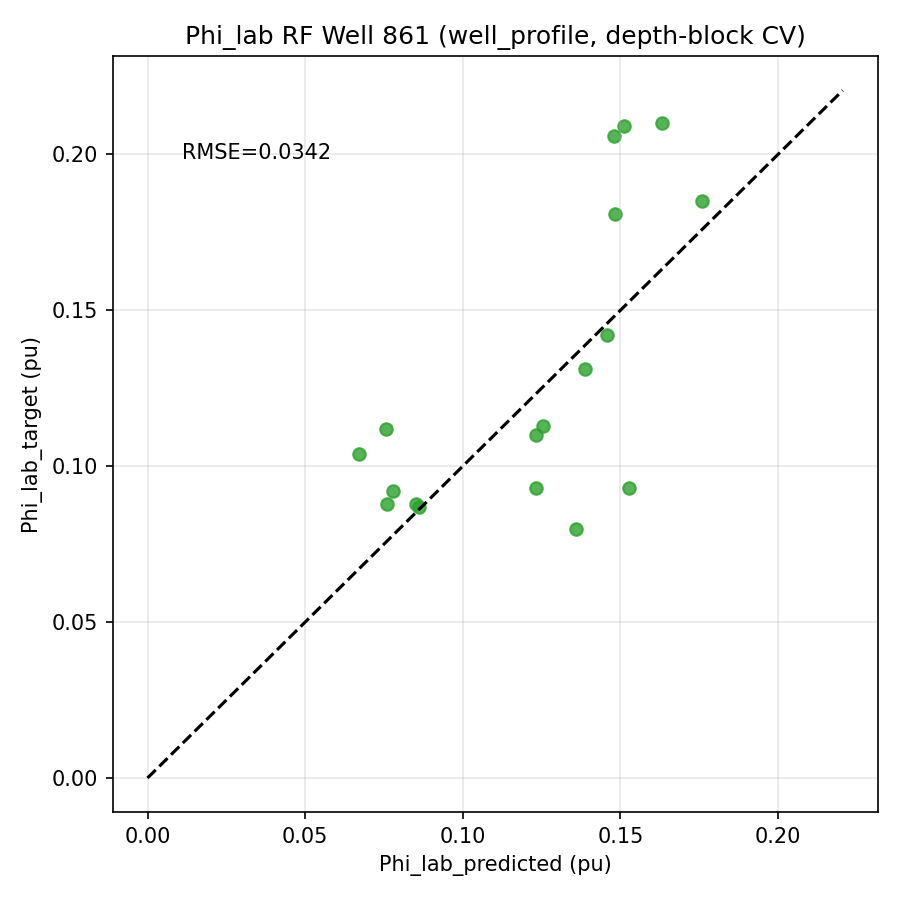
\includegraphics[width=\linewidth]{figures/fig_phi_rf_pred_vs_obs}
    \caption{Predito versus observado (divisão 80/20, ilustrativo).}
    \label{fig:phi_pred}
  \end{subfigure}
  \hfill
  \begin{subfigure}[t]{0.48\linewidth}
    \centering
    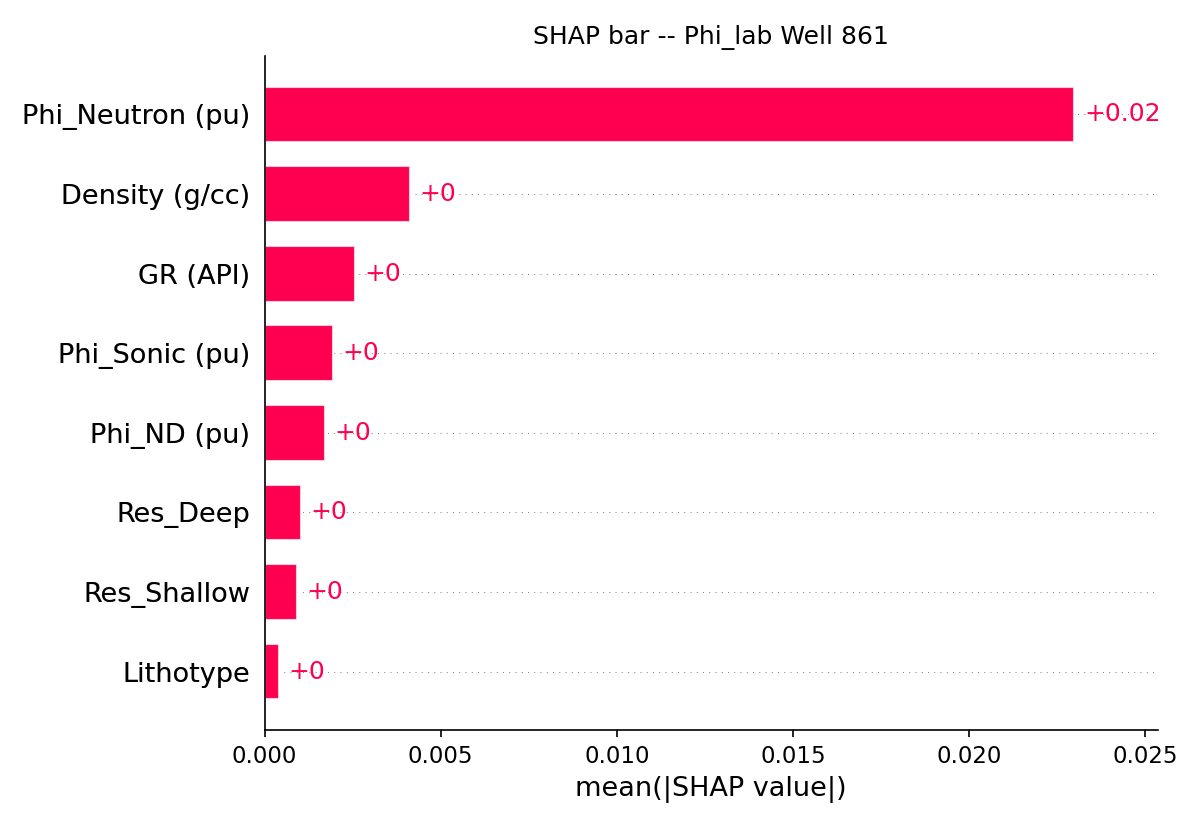
\includegraphics[width=\linewidth]{figures/fig_phi_shap_bar}
    \caption{Contribuição das curvas (SHAP).}
    \label{fig:phi_shap}
  \end{subfigure}
  \caption{Complementos do RF para \philab{} (não substituem as figuras OOF).}
  \label{fig:phi_rf_panel}
\end{figure}

A Figura~\ref{fig:phi_rf_panel} complementa a analise em dois painéis
secundários.

\emph{Painel (a)---predito versus observado:}
Os pontos deveriam alinhar-se à diagonal (predição perfeita).
O agrupamento geral ao longo da diagonal indica que o RF captura a tendência
de porosidade, mas com dispersão visível---consistente com $R^2 = 0{,}146$
na validação por blocos.
Esta figura usa divisão aleatória 80/20 e tende a parecer melhor do que a
validação por blocos; por isso a tratamos apenas como ilustração.

\emph{Painel (b)---importância SHAP:}
As barras indicam quais curvas mais influenciam as predições do RF.
Espera-se que \phiN{}, \phiND{} e $\rho_b$
dominem, pois são as curvas com maior correlação com \philab{}
(Tabela~\ref{tab:corr_phi}).
Se curvas de litologia (GR, litotipo) aparecerem com peso relevante, isso
sugere que o modelo usa informação litológica para ajustar a porosidade
estimada---comportamento razoável em carbonatos com múltiplos litotipos.

\subsection{FZI de laboratório: falha na generalização}

O RF para \fzilab{} (Tabela~\ref{tab:fzi_folds}) confirma o
colapso no bloco~1, onde predomina \emph{Grainstone} (litotipo~1).
Uma divisão aleatória 80/20 daria $R^2 \approx 0{,}17$---resultado
enganoso, pois mistura profundidades semelhantes entre treino e teste.

\begin{table}[H]
  \centering
  \caption{RF para \fzilab{}: resultado em cada bloco de teste.}
  \label{tab:fzi_folds}
  \begin{tabular}{ccrr}
    \toprule
    Bloco & Prof.\ teste (m) & RMSE & $R^2$ \\
    \midrule
    0 & 5206--5214 & 1,30 & $-0{,}015$ \\
    1 & 5215--5223 & 2,14 & $-1{,}945$ \\
    2 & 5225--5234 & 2,00 & $-0{,}496$ \\
    \midrule
    Média & -- & 1,81 & $-0{,}819$ \\
    \bottomrule
  \end{tabular}
\end{table}

Na Tabela~\ref{tab:fzi_folds}, o colapso no bloco~1 ($R^2 = -1{,}945$) é o resultado mais relevante.
Este bloco concentra \emph{Grainstone} (19 de 29 amostras, litotipo~1) e tem FZI médio
relativamente baixo ($\overline{\mathrm{FZI}} = 1{,}25$), mas com variabilidade
interna que o perfil não captura.
O RMSE de 2,14 neste bloco representa erro substancial frente à faixa típica
de FZI no poço.
No bloco~0, o $R^2 \approx 0$ indica desempenho equivalente à média; no
bloco~2, $R^2 = -0{,}496$ confirma falha também no intervalo mais permeável.

Compare com o resultado enganoso de uma divisão aleatória 80/20
($R^2 \approx 0{,}17$): esse valor \emph{superestima} a capacidade preditiva
porque amostras do bloco~1 aparecem tanto no treino quanto no teste.
A validação por blocos expõe a fragilidade real do modelo.

\section{Resultados nos plugs com microCT}
\label{sec:ctplugs}

Com apenas 10 amostras, os resultados devem ser interpretados com
cautela.
A Tabela~\ref{tab:ctplugs} reporta o $R^2$ global das predições
OOF do RF.

Para \fzilab{}, usar somente curvas de perfil superou incluir descritores
de microCT.
Para \philab{}, ambos os modos deram $R^2$ negativo.
A Figura~\ref{fig:ct_fzi} mostra o ajuste plug a plug para FZI.

\begin{table}[H]
  \centering
  \caption{RF nos 10 plugs: $R^2$ global (validação LOPO).}
  \label{tab:ctplugs}
  \begin{tabular}{lrr}
    \toprule
    Alvo & Somente perfil & Perfil + microCT \\
    \midrule
    FZI\_lab & 0,151 & 0,116 \\
    Phi\_lab (pu) & $-0{,}334$ & $-0{,}466$ \\
    \bottomrule
  \end{tabular}
\end{table}

\begin{figure}[H]
  \centering
  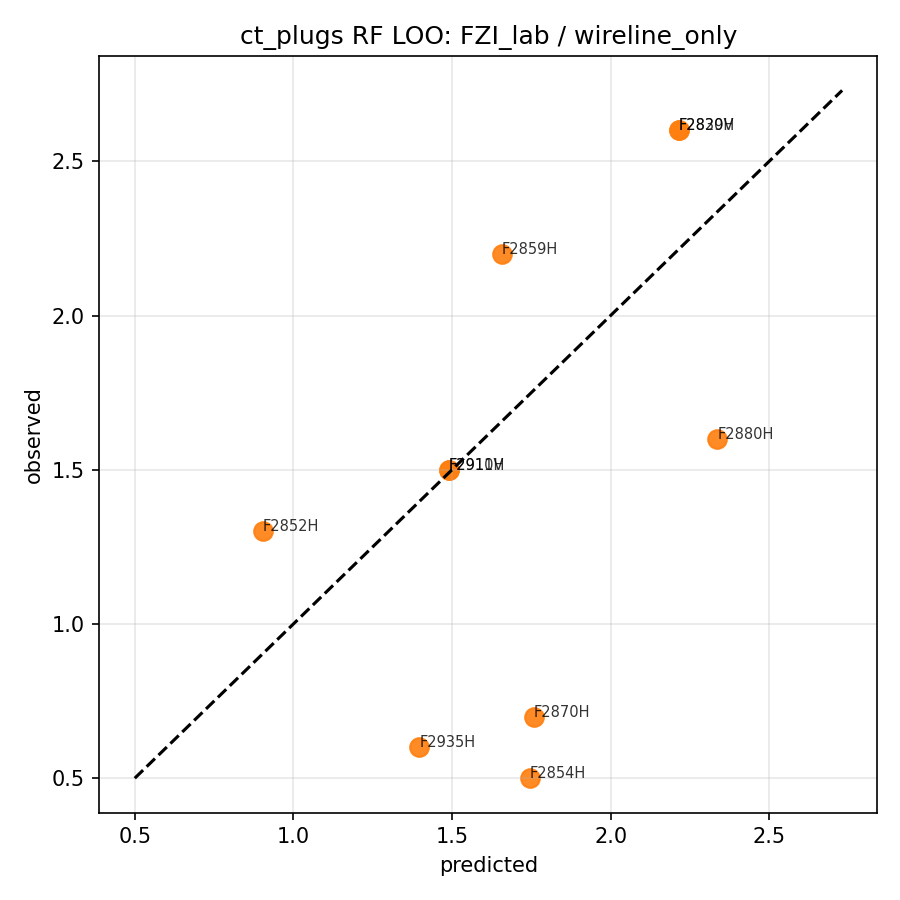
\includegraphics[width=0.72\linewidth]{figures/fig_ct_plugs_fzi_wireline}
  \caption{LOPO-RF para \fzilab{} nos plugs: predito versus
           observado (somente curvas de perfil).}
  \label{fig:ct_fzi}
\end{figure}

Lidos em conjunto, os resultados nos dez plugs exigem cautela extrema na extrapolacao ao perfil completo.

\emph{FZI nos plugs} ($R^2 = 0{,}151$ somente perfil; $0{,}116$ com microCT):
o valor positivo fraco sugere que, com apenas dez amostras, o RF captura
alguma tendência de FZI a partir das curvas de perfil adjacentes a cada plug.
Porém, incluir descritores de microCT \emph{piorou} levemente o resultado
(0,151 $\rightarrow$ 0,116)---provavelmente por overfitting: sete variáveis
extras em um conjunto de dez amostras aumentam o risco de o modelo memorizar
padrões específicos de cada plug em vez de aprender relações gerais.

Na Figura~\ref{fig:ct_fzi}, cada ponto corresponde a um plug identificado
individualmente.
A dispersão em torno da diagonal indica predições com erro plug a plug;
não há evidência de ajuste sistemático preciso.
Com dez pontos, um único plug mal predito altera fortemente o $R^2$ global.

\emph{Porosidade nos plugs} ($R^2 = -0{,}334$ somente perfil; $-0{,}466$ com
microCT): ambos negativos.
Os dez plugs não representam bem a variabilidade das 87 amostras do perfil
completo---a porosidade dos plugs pode diferir da porosidade média do
intervalo perfurado nas mesmas profundidades.
Este resultado confirma que a análise nos dez plugs não substitui o
perfil completo de 87 amostras para estimar porosidade ao longo do poço.

O $R^2$ positivo fraco de FZI nos dez plugs \emph{não} significa que o
modelo generaliza para as 87 amostras do perfil completo: o conjunto de
plugs é pequeno e cada plug removido altera bastante o resultado.

\section{Alternativas de modelo (Etapa~1e)}
\label{sec:alternativas}

\subsection{Porosidade: modelos mais simples versus RF}

Testamos se um modelo mais simples poderia igualar o RF para
\philab{}.
A Tabela~\ref{tab:phi_models} e a Figura~\ref{fig:phi_models} comparam
Ridge (regressão linear com penalização), GAM (modelo aditivo
generalizado, aqui aproximado por splines + Ridge) e o RF.

Nenhuma alternativa superou o RF.
O GAM foi aproximado por splines cubicas seguidas de regressão Ridge,
por indisponibilidade da biblioteca especializada no ambiente de execução.

\begin{table}[H]
  \centering
  \caption{\philab{}: comparação entre RF, GAM e Ridge.}
  \label{tab:phi_models}
  \begin{tabular}{lrr}
    \toprule
    Modelo & RMSE médio (pu) & $R^2$ médio \\
    \midrule
    RF (referência) & 0,033 & \textbf{0,146} \\
    GAM (spline+Ridge) & 0,036 & $-0{,}052$ \\
    Ridge & 0,037 & $-0{,}261$ \\
    \bottomrule
  \end{tabular}
\end{table}

\begin{figure}[H]
  \centering
  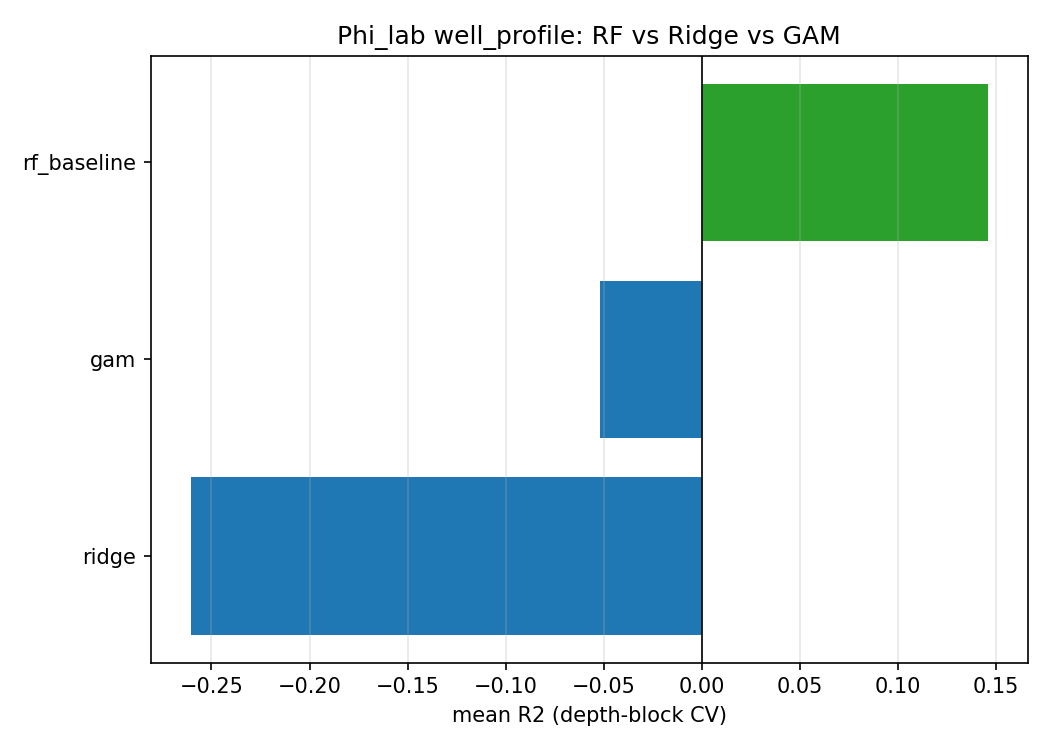
\includegraphics[width=0.78\linewidth]{figures/fig_phi_model_comparison}
  \caption{$R^2$ médio para \philab{}: RF, GAM e Ridge.}
  \label{fig:phi_models}
\end{figure}

O RF permanece superior: $R^2 = 0{,}146$ contra $-0{,}052$ (GAM) e $-0{,}261$
(Ridge).
O Ridge, sendo um modelo linear, assume relação fixa entre curvas e
porosidade---o que falha quando a relação muda entre blocos litológicos
(Tabela~\ref{tab:depthblocks}).
O GAM permite relações não lineares por curva, mas a implementação
disponível (splines + Ridge) não superou o RF, possivelmente porque 87
amostras são poucas para estimar curvas flexíveis com estabilidade entre
blocos.
Na Figura~\ref{fig:phi_models}, a barra do RF é a única acima da linha de
referência ($R^2 = 0$); Ridge e GAM ficam abaixo, confirmando que modelos
mais simples não compensam a limitação de informação do perfil.

\subsection{Classificação de HFU}

A Tabela~\ref{tab:hfu_class} resume a acurácia das predições OOF.
A regressão logística com pesos balanceados superou o RF balanceado,
mas a acurácia global ($\approx 36\%$) continua modesta: em quatro
classes, o acaso corresponde a cerca de 25\%.

A \emph{acurácia balanceada} dá peso igual a cada classe, evitando que
o modelo pareça bom apenas por acertar a classe majoritária (HFU1).

\begin{table}[H]
  \centering
  \caption{Classificação de HFU (validação por blocos,
           predições OOF).}
  \label{tab:hfu_class}
  \begin{tabular}{lrrr}
    \toprule
    Modelo & Acurácia & Acurácia balanceada & F1 macro \\
    \midrule
    Logística balanceada & 0,356 & 0,220 & 0,217 \\
    RF balanceado & 0,299 & 0,179 & 0,161 \\
    \bottomrule
  \end{tabular}
\end{table}

\begin{figure}[H]
  \centering
  \begin{subfigure}[t]{0.48\linewidth}
    \centering
    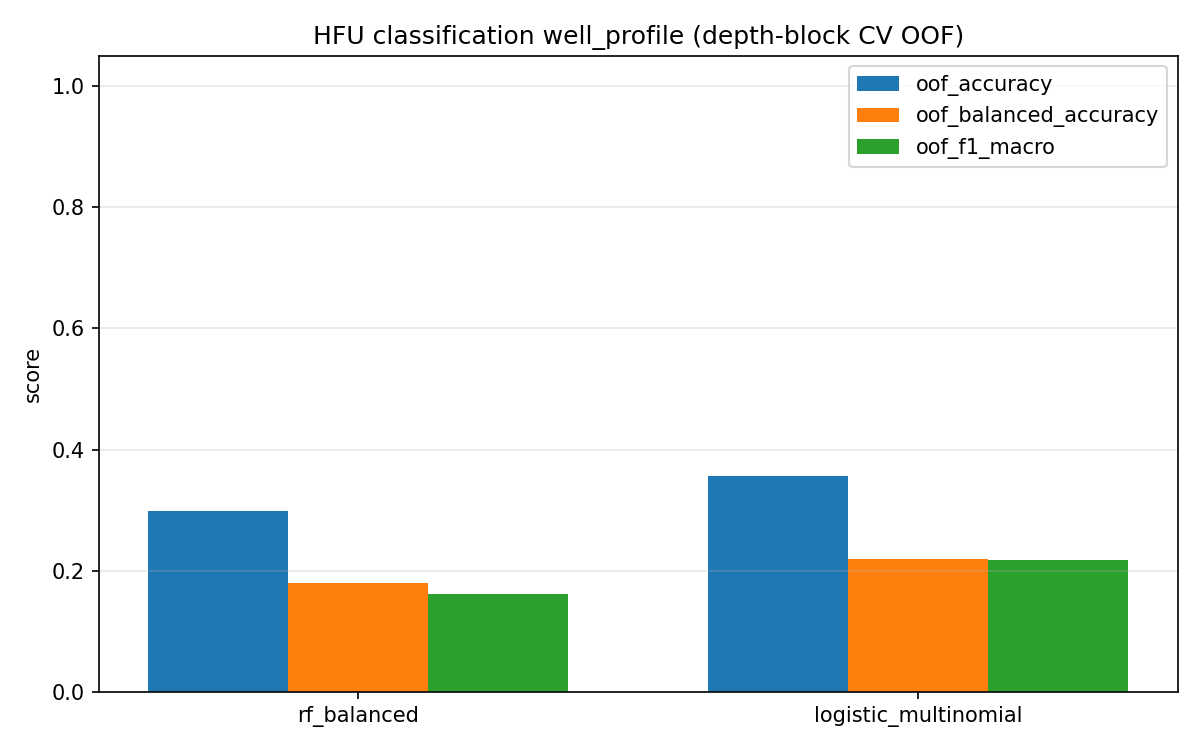
\includegraphics[width=\linewidth]{figures/fig_hfu_classifier_oof}
    \caption{Métricas por modelo.}
    \label{fig:hfu_metrics}
  \end{subfigure}
  \hfill
  \begin{subfigure}[t]{0.48\linewidth}
    \centering
    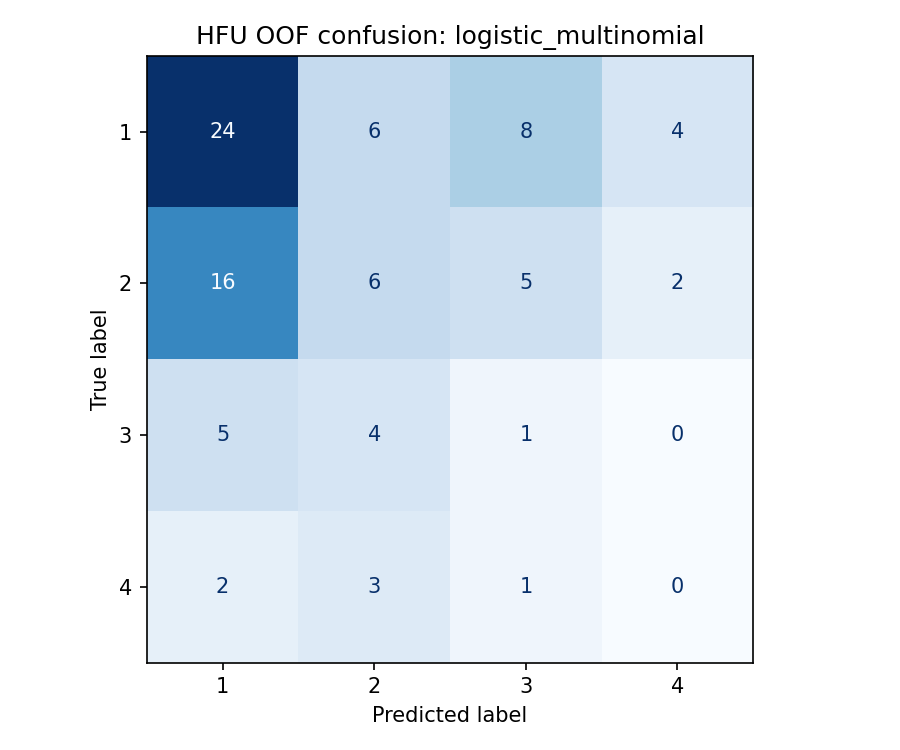
\includegraphics[width=\linewidth]{figures/fig_hfu_confusion_logistic}
    \caption{Matriz de confusão (logística).}
    \label{fig:hfu_confusion}
  \end{subfigure}
  \caption{Classificação de HFU no perfil completo.}
  \label{fig:hfu_panel}
\end{figure}

A logística balanceada supera o RF em todas as métricas da Figura~\ref{fig:hfu_metrics}, embora o desempenho global continue modesto.

\emph{Acurácia global} (logística: 35,6\%; RF: 29,9\%): a regressão
logística acerta pouco mais de um terço das amostras.
Para quatro classes, o chute aleatório daria $\sim$25\%; o ganho sobre o
acaso é de apenas 10 pontos percentuais---desempenho modesto.

\emph{Acurácia balanceada} (logística: 22,0\%; RF: 17,9\%): ao dar peso
igual a cada HFU, o desempenho cai abaixo do acaso (25\%).
Isso indica que o modelo tem dificuldade especial nas classes minoritárias
HFU3 ($n=10$) e HFU4 ($n=6$).

\emph{F1 macro} (logística: 0,217; RF: 0,161): métrica que combina
precisão e revocação por classe; valores próximos de 0,2 confirmam
desempenho fraco e heterogêneo entre HFUs.

Na Figura~\ref{fig:hfu_metrics}, a logística supera o RF em todas as
métricas---modelos lineares tendem a generalizar melhor com poucos dados
e classes desbalanceadas.
Na Figura~\ref{fig:hfu_confusion}, a matriz de confusão mostra onde ocorrem
os erros: espera-se confusão entre HFU1 e HFU2 (classes mais frequentes e
petrofísicamente mais próximas), e poucos acertos em HFU3 e HFU4.
Para a Etapa~2, a HFU de laboratório deve ser priorizada; a predição
automática serve apenas como recurso auxiliar onde não houver amostra de
laboratório.

\section{CLP-CSGM com laboratório esparso nos plugs (Etapa~1f)}
\label{sec:clp}

\subsection{Motivação e pergunta científica}

Na Etapa~1d, o RF responde à pergunta pontual: \emph{wireline sozinho
prevê \philab{} em cada profundidade?}
Com $R^2 \approx 0{,}15$ (Tabela~\ref{tab:phi_folds}), o perfil já
carrega sinal útil, porém com erro heterogêneo entre blocos.

A Etapa~1f pergunta de forma complementar:

\begin{quote}
\emph{Com wireline denso ao longo da janela ($\mathbf{u}$) e \philab{}
medida apenas nos dez plugs ($\mathbf{b}$), é possível reconstruir a
\emph{curva} $\phi(z)$ ao longo do intervalo de forma estruturalmente
correta, sem tratar laboratório como feature de entrada?}
\end{quote}

O arcabouço CLP-CSGM (Compressed Learning Problem com generative
prior no espaço latente) impõe consistência esparsa
$\|M\,G(\zvec)-\mathbf{b}\|_2^2$ entre a curva reconstruída
$G(\zvec)$ e as amarras de laboratório, em vez de concatenar \philab{}
ao vetor de features---o que causaria vazamento informacional na
validação.

Neste poço, o desafio é severo: apenas dez plugs em 87 amostras e oito
profundidades únicas com amarra fixa; o RF pontual já é forte no bloco
superior.
A motivação do experimento não é substituir o RF por default, e sim
testar se amarras esparsas de laboratório \emph{refinam} o perfil quando
a formulação inversa é honesta.

\subsection{Notação por janela deslizante}

Seguimos janelas de comprimento $L=16$ amostras e passo unitário ao
longo das 87 profundidades.
Para cada janela:

\begin{itemize}
  \item $\mathbf{y}\in\mathbb{R}^{L}$: curva de \philab{} na janela
        (alvo de referência na validação, não usada em $\mathbf{u}$).
  \item $\mathbf{u}$: oito curvas wireline na mesma janela (GR, densidade,
        resistividades, $\phi_{\mathrm{N}}$, $\phi_{\mathrm{S}}$, \phiND{},
        litotipo), idênticas à Etapa~1d.
  \item $M\in\{0,1\}^{m\times L}$: matriz de subsampling por
        \emph{coordenada}; $m$ é o número de plugs dentro da janela
        (máscara fixa, não amostragem aleatória $\rho$).
  \item $G(\zvec)=\mathrm{Dec}(\zvec)$: decodificador do autoencoder
        (AE) treinado offline nas janelas de treino do fold.
  \item $\zzero$: código latente de prior condicional.
  \item $\lambda>0$: peso de regularização Tikhonov no latente.
\end{itemize}

A validação repete o protocolo de três blocos contíguos da
Seção~\ref{sec:protocolo}: em cada fold, o RF e o AE só veem dados de
treino; as métricas OOF comparam predições pontuais nas 87 profundidades
com o mesmo RF de referência.

\subsection{Problema inverso CLP-CSGM (formulação base)}

Dado $\mathbf{b}$ e $M$, o recuperador CSGM resolve, para cada janela de
teste,
\begin{equation}
  \zvec^{\ast}
  =
  \arg\min_{\zvec}
  \frac{1}{m}\,\|M\,G(\zvec)-\mathbf{b}\|_2^2
  +
  \lambda\,\|\zvec-\zzero\|_2^2,
  \label{eq:clp_inverse}
\end{equation}
onde $m$ é o número de linhas de $M$ (plugs na janela).
O balanço entre o termo de dados e o prior latente, o caso $m=0$ e a
leitura janela a janela nas variantes~A e~B são detalhados na
Seção~\ref{sec:clp_balance}.

A âncora $\zzero$ \emph{não} é apenas chute inicial do otimizador: ela
entra explicitamente no custo \eqref{eq:clp_inverse} e equilibra
aderência às medidas esparsas versus permanência próxima ao prior
latente.
O hiperparâmetro $\lambda$ é escolhido por grade no conjunto de
validação interno de cada fold (20\% do pool de treino).

A curva predita na janela depende da variante (Seção~\ref{sec:clp_variants}).
Predições de janelas sobrepostas são fundidas por média uniforme ao longo
da profundidade (mesma regra de \emph{stitching} OOF usada nas figuras de
\philab{}).

\subsection{Balanço do custo inverso e papel de \texorpdfstring{$m$}{m}}
\label{sec:clp_balance}

A equação \eqref{eq:clp_inverse} combina duas fontes de informação com
papéis distintos.
O termo de dados
$\|M\,G(\zvec)-\mathbf{b}\|_2^2$
impõe consistência com o \textbf{laboratório esparso} nos índices
selecionados por $M$: em cada coordenada-plug, a curva reconstruída deve
aproximar o valor prescrito em $\mathbf{b}$.
O termo de prior
$\lambda\|\zvec-\zzero\|_2^2$
penaliza desvios de um \textbf{centro latente} $\zzero$ que resume a
crença \emph{a priori} antes de olhar as amarras daquela janela---seja
$h(\mathbf{u})$, $\mathrm{Enc}(\widehat{\phi}_{\mathrm{RF}})$ ou
$\mathrm{Enc}(\mathbf{0})$, conforme a variante.

Nenhum dos dois termos ``carrega a informação'' sozinho em todas as
situações: quem domina depende de $m$, de $\lambda$ e de como a predição
final é montada (somente $G(\zvec)$ na variante~A versus
$\widehat{\phi}_{\mathrm{RF}}+G(\zvec)$ na variante~B).
A Tabela~\ref{tab:clp_m_balance} resume os regimes.

\begin{table}[H]
  \centering
  \caption{Regimes do inverso \eqref{eq:clp_inverse} por número de plugs
           na janela ($m$) e variante.}
  \label{tab:clp_m_balance}
  \small
  \begin{tabular}{p{1.2cm}p{4.5cm}p{4.8cm}p{3.8cm}}
    \toprule
    $m$ & Termo ativo & Otimização em $\zvec$? & Papel dominante \\
    \midrule
    $0$ &
      só $\lambda\|\zvec-\zzero\|^2$;
      $M$ e $\mathbf{b}$ vazios &
      não; $\zvec=\zzero$ &
      prior latente (e, na B, $\widehat{\phi}_{\mathrm{RF}}$) \\
    $\ge 1$ &
      dados + prior &
      sim; trade-off via $\lambda$ &
      lab nos plugs + prior + AE ao longo de $L$ \\
    \bottomrule
  \end{tabular}
\end{table}

\subsubsection{Caso \texorpdfstring{$m=0$}{m=0}: ausência de plug na janela}

Com dez plugs em 87 amostras e janelas de $L=16$, \emph{muitas} janelas
deslizantes não contêm nenhuma profundidade-plug: para elas, $M$ tem
dimensão $0\times L$ e $\mathbf{b}\in\mathbb{R}^0$.
O termo de dados desaparece, porque
$\|M\,G(\zvec)-\mathbf{b}\|_2^2=0$ para qualquer $\zvec$.
O recuperador \emph{não executa} iterações de gradiente: fixa
$\zvec=\zzero$ e devolve $G(\zzero)$ decodificado.

Esse mecanismo é \textbf{comum às variantes A e~B}.
A diferença está no \emph{significado} de $\zzero$ e na fórmula da
saída---não na presença ou ausência do termo de dados.

\paragraph{Variante~A com $m=0$.}
Com $\zzero=\mathrm{Enc}(\widehat{\phi}_{\mathrm{RF}})$ no
AE$_{\phi}$,
\begin{equation}
  \widehat{\phi}
  =
  G_{\phi}(\zzero)
  =
  G_{\phi}\!\left(\mathrm{Enc}(\widehat{\phi}_{\mathrm{RF}})\right).
  \label{eq:clp_a_m0}
\end{equation}
Trata-se de \emph{reconstruir} a curva RF passando pelo autoencoder
treinado em $\phi_{\mathrm{lab}}$.
Em geral,
$G_{\phi}(\mathrm{Enc}(\widehat{\phi}_{\mathrm{RF}}))
\not\approx \widehat{\phi}_{\mathrm{RF}}$
ponto a ponto: o encode--decode introduz erro de reconstrução e o
manifold de $\phi_{\mathrm{lab}}$ não coincide com o das predições RF.
Mesmo ``só prior'', a variante~A \textbf{não} devolve o RF cru.

\paragraph{Variante~B com $m=0$.}
Com $\zzero=\mathrm{Enc}(\mathbf{0})$ no AE$_{\delta}$,
\begin{equation}
  \widehat{\phi}
  =
  \widehat{\phi}_{\mathrm{RF}}
  +
  G_{\delta}(\zzero)
  \approx
  \widehat{\phi}_{\mathrm{RF}} + \mathbf{0}.
  \label{eq:clp_b_m0}
\end{equation}
Aqui $\mathrm{Enc}(\mathbf{0})$ \emph{é} a âncora latente: codifica
``resíduo nulo'' no espaço em que o AE foi treinado (após
padronização).
Não se fixa $\zvec=\mathbf{0}$ literalmente em $\mathbb{R}^k$---isso
não garantiria $G_{\delta}(\mathbf{0})=\mathbf{0}$ em escala física.
A baseline wireline $\widehat{\phi}_{\mathrm{RF}}$ entra
\textbf{explicitamente} na soma; o prior só controla a correção
$\widehat{\deltaphi}$, que colapsa quando não há amarra.

\subsubsection{Caso \texorpdfstring{$m\ge 1$}{m>=1}: plug(s) dentro da janela}

Quando há pelo menos um plug, $\mathbf{b}$ é não vazio e o otimizador
ajusta $\zvec$ equilibrando dados e prior.
O hiperparâmetro $\lambda$, escolhido por grade na validação interna,
controla esse balanço:
\begin{itemize}
  \item $\lambda$ \textbf{grande}: o inverso permanece próximo de $\zzero$;
        a curva fica suave e pode subajustar os plugs.
  \item $\lambda$ \textbf{pequeno}: o termo $\|M\,G(\zvec)-\mathbf{b}\|^2$
        pesa mais; a reconstrução aproxima $\mathbf{b}$ nos índices medidos.
\end{itemize}

Importante: $M$ seleciona apenas $m$ coordenadas, mas $G(\zvec)$ é uma
\emph{curva completa} de comprimento $L$.
O autoencoder acopla todos os índices da janela: a correção imposta no
plug propaga-se, via $G$ e via $\lambda$, às profundidades vizinhas
dentro da mesma janela.

Na variante~A, $\mathbf{b}=M\,\phi_{\mathrm{lab}}$ ancora $\phi$ absoluta.
Na variante~B, $\mathbf{b}=M(\phi_{\mathrm{lab}}-\widehat{\phi}_{\mathrm{RF}})$
ancora o \emph{desvio} do RF; a saída
$\widehat{\phi}=\widehat{\phi}_{\mathrm{RF}}+G_{\delta}(\zvec^{\ast})$
ainda soma a baseline em toda a janela.

\subsubsection{Leitura no perfil completo (87 profundidades)}

O perfil OOF final funde janelas sobrepostas por média uniforme.
Cada profundidade é coberta por várias janelas, algumas com $m=0$ e
outras com $m\ge 1$.
Por isso o comportamento \emph{global} é uma mistura:
\begin{itemize}
  \item trechos onde predominam janelas com $m=0$ tendem a seguir o
        \emph{default} do prior (e, na B, o RF);
  \item trechos próximos a plugs recebem contribuição de janelas com
        $m\ge 1$, nas quais o laboratório altera $\zvec^{\ast}$ e, por
        extensão, a curva ao longo de $L$.
\end{itemize}

No poço~861, o laboratório só fixa oito profundidades com amarra; a
maior parte do intervalo é coberta sobretudo por janelas sem plug.
Isso explica por que a variante~B quase reproduz o RF globalmente
(Tabela~\ref{tab:clp_vs_rf_global}): a informação wireline já está em
$\widehat{\phi}_{\mathrm{RF}}$, e $\|z-z_0\|^2$ só modula \emph{quanto}
desviar---não reconstrói $\phi$ do zero como na variante~A.
A degradação da variante~A ($\Delta$RMSE $=+0{,}005$~pu) reflete,
em parte, janelas $m=0$ em que $G_{\phi}(\mathrm{Enc}(\widehat{\phi}_{\mathrm{RF}}))$
se afasta do RF pontual, e janelas $m\ge 1$ em que $G_{\phi}(\zvec^{\ast})$
suaviza ou desloca a curva inteira.

\paragraph{O que o leitor deve reter.}
O prior $\|z-z_0\|^2$ define o \textbf{comportamento padrão} de cada
janela quando o laboratório não fala ($m=0$) ou fala pouco ($\lambda$
grande).
Ele \emph{não} substitui, em geral, a informação wireline---exceto
indiretamente via $\zzero$.
Na variante~B, a informação wireline dominante está em
$\widehat{\phi}_{\mathrm{RF}}$; o inverso latente estima apenas o
resíduo local exigido por $\mathbf{b}$ nos plugs.

\subsection{Papel do prior latente \texorpdfstring{$\zzero$}{z0}:
três construções e por que importam}
\label{sec:clp_z0}

O termo $\lambda\|\zvec-\zzero\|_2^2$ em \eqref{eq:clp_inverse} penaliza
desvios do código latente em relação a um \emph{centro de prior}.
A escolha de $\zzero$ define qual curva (ou correção) o inverso prefere
quando as amarras $\mathbf{b}$ são escassas ou ausentes ($m$ pequeno ou
$m=0$).
Não se trata de mera inicialização numérica: $\zzero$ permanece no
objetivo durante toda a otimização.

No arcabouço CLP-CSGM original, o prior condicional mapeia informação
abundante para o latente:
\begin{equation}
  \zzero = h(\mathbf{u}),
  \label{eq:clp_h_u}
\end{equation}
com $h$ Ridge ou rede rasa treinada para aproximar
$\mathrm{Enc}(\mathrm{AE},\mathbf{y})$ a partir de $\mathbf{u}$
\emph{somente nos dados de treino do fold}.
Essa é a construção \textbf{(I) $h(\mathbf{u})$}, usada nas variantes
Ridge/MLP da Etapa~1f.

\paragraph{Por que (I) não basta no poço~861.}
O mapeamento $h(\mathbf{u})$ aprende um centro latente a partir do
wireline, mas a curva decodificada $G(\zzero)$ não coincide, em geral,
com a melhor predição pontual de \philab{} já obtida na Etapa~1d.
Na prática, Ridge/MLP em $h(\mathbf{u})$ com AE em $\phi$ absoluta
produziram RMSE médio por janela de 0,049--0,051~pu (três \emph{seeds}),
sistematicamente acima do RF pontual (0,036~pu na comparação OOF
alinhada).
Ou seja: priorizar um $\zzero$ derivado só de $\mathbf{u}$ no espaço
latente de $\phi$ \emph{não garante} que a reconstrução final herde a
qualidade do RF, porque $G$ foi treinado no manifold de $\phi_{\mathrm{lab}}$
e não no manifold das predições RF.

\paragraph{Construção (II): $\zzero=\mathrm{Enc}(\widehat{\phi}_{\mathrm{RF}})$.}
Para alinhar o prior ao melhor baseline wireline, codifica-se no AE a
\emph{curva} RF na janela (vetor $\widehat{\phi}_{\mathrm{RF}}\in\mathbb{R}^L$,
não o vetor de features $\mathbf{u}$):
\begin{equation}
  \zzero
  =
  \mathrm{Enc}\!\left(
    \mathrm{AE}_{\phi},\;
    \widehat{\phi}_{\mathrm{RF}}
  \right).
  \label{eq:clp_enc_rf}
\end{equation}
Note a distinção conceitual: $h(\mathbf{u})$ opera no espaço de
\emph{entradas} (dimensão das features concatenadas na janela); já
$\mathrm{Enc}(\widehat{\phi}_{\mathrm{RF}})$ opera no \emph{espaço de
saída} em que o AE foi treinado (curvas de $\phi$ de comprimento $L$).
Não existe, nesta pipeline, um $\mathrm{Enc}(\mathbf{u})$---o encoder
consome curvas-alvo, não perfis wireline isolados.

A intenção de (II) é puxar $\zvec$ para um latente cujo decode reproduza
aproximadamente a curva RF \emph{no manifold de $\phi$}.
Porém a predição final é $G(\zvec^{\ast})$ inteira: o RF entra só na
regularização, não na soma final.
Quando $\lambda$ é pequeno ou há poucos plugs, $G(\zvec^{\ast})$ pode
afastar-se da curva RF que motivou $\zzero$, reconstruindo $\phi$ absoluta
com suavização do AE---daí a degradação observada na variante~A
(Tabela~\ref{tab:clp_vs_rf_global}).

\paragraph{Construção (III): $\zzero=\mathrm{Enc}(\mathbf{0})$ no AE de
resíduos.}
Na variante residual, o AE modela $\deltaphi$, não $\phi$ absoluta.
O prior neutro é \emph{correção nula}:
\begin{equation}
  \zzero
  =
  \mathrm{Enc}\!\left(
    \mathrm{AE}_{\delta},\;
    \mathbf{0}
  \right),
  \label{eq:clp_enc_zero}
\end{equation}
com $\mathbf{0}\in\mathbb{R}^L$ antes da padronização (resíduo médio
nulo na escala física).

\emph{Por que não usar $h(\mathbf{u})$ na variante~B?}
O wireline já entra explicitamente em $\widehat{\phi}_{\mathrm{RF}}$,
que é a baseline \emph{fora} do inverso \eqref{eq:clp_inverse}.
Definir $\zzero=h(\mathbf{u})$ no AE de $\deltaphi$ misturaria dois papéis:
(i)~informação já absorvida pelo RF na baseline; (ii)~centro latente para
$\deltaphi$, cuja interpretação física seria opaca (wireline não é
resíduo).
O prior $\mathrm{Enc}(\mathbf{0})$ expressa diretamente a hipótese
\emph{``não corrigir o RF''} quando não há amarra de laboratório; com
$m=0$, $\widehat{\deltaphi}\approx\mathbf{0}$ e
$\widehat{\phi}\approx\widehat{\phi}_{\mathrm{RF}}$.

\emph{Por que não $\mathrm{Enc}(\widehat{\phi}_{\mathrm{RF}})$ no AE
$\delta$?}
Esse código corresponderia a um resíduo \emph{não nulo} no manifold do
AE---ou seja, a baseline deixaria de ser correção zero e o inverso
partiria de um viés sistemático em $\deltaphi$, anulando a decomposição
\eqref{eq:clp_residual_decomp}.

A Tabela~\ref{tab:clp_z0_roles} resume os três centros latentes e o
efeito esperado sobre a predição.

\begin{table}[H]
  \centering
  \caption{Três construções de $\zzero$ no CLP-CSGM e papel na predição
           de \philab{} (poço~861).}
  \label{tab:clp_z0_roles}
  \small
  \begin{tabular}{p{2.2cm}p{3.8cm}p{4.2cm}p{3.8cm}}
    \toprule
    ID & Definição de $\zzero$ & Espaço do AE & Efeito quando $m=0$ \\
    \midrule
    (I) &
      $h(\mathbf{u})$ Ridge/MLP &
      $\phi_{\mathrm{lab}}$ &
      $G(\zzero)$: curva $\phi$ genérica do wireline, não necessariamente RF \\
    (II) &
      $\mathrm{Enc}(\widehat{\phi}_{\mathrm{RF}})$ &
      $\phi_{\mathrm{lab}}$ &
      $G(\zzero)\approx\widehat{\phi}_{\mathrm{RF}}$ no manifold $\phi$,
      mas $\widehat{\phi}=G(\zvec^{\ast})$ pode divergir \\
    (III) &
      $\mathrm{Enc}(\mathbf{0})$ &
      $\deltaphi$ &
      $\widehat{\deltaphi}\approx\mathbf{0}$,
      $\widehat{\phi}=\widehat{\phi}_{\mathrm{RF}}$ \\
    \bottomrule
  \end{tabular}
\end{table}

Em síntese: (I) é o prior CLP canônico, insuficiente quando o RF pontual
já é forte; (II) melhora o \emph{centro latente} em $\phi$, mas não
ancora a \emph{resposta final}; (III) alinha prior, baseline e objetivo
---corrigir só o que o laboratório esparso exige.

\subsection{Variantes experimentais}
\label{sec:clp_variants}

\subsubsection{Variante A: prior RF no espaço de \philab{} (CLP clássico)}

Esta variante combina AE em $\phi$ absoluta com a construção~(II):
$\zzero=\mathrm{Enc}(\widehat{\phi}_{\mathrm{RF}})$ conforme
\eqref{eq:clp_enc_rf}.
\begin{equation}
  \mathbf{b}
  =
  M\,\mathbf{y}
  =
  M\,\phi_{\mathrm{lab}}.
  \label{eq:clp_b_abs}
\end{equation}

A predição final é $\widehat{\mathbf{y}}=G(\zvec^{\ast})$---ou seja, o
RF entra somente em $\zzero$ e \emph{não} na resposta final.
Interpretação: o CSGM tenta \emph{reconstruir a curva inteira} de
\philab{}, puxada ao RF no latente mas livre para se afastar dele na
decodificação quando $\lambda$ é pequeno ou quando poucas amarras
constroem $\mathbf{b}$.

Variantes com construção~(I), $h(\mathbf{u})$ Ridge ou MLP, estão
documentadas na Tabela~\ref{tab:clp_z0_roles}; não superaram o RF
pontual (RMSE por janela $\approx 0{,}049$--0,051~pu).

\subsubsection{Variante B: CLP residual sobre o RF}

Quando o RF já explica boa parte da variância, reconstruir $\phi$
absoluta força o inverso a repetir trabalho que o wireline resolve.
A variante~B usa a construção~(III) da
Seção~\ref{sec:clp_z0} e \emph{reparametriza} o problema:

\begin{equation}
  \deltaphi
  =
  \phi_{\mathrm{lab}} - \widehat{\phi}_{\mathrm{RF}},
  \qquad
  \widehat{\phi}
  =
  \widehat{\phi}_{\mathrm{RF}} + \widehat{\deltaphi}.
  \label{eq:clp_residual_decomp}
\end{equation}

\textbf{Treino do AE.}
O autoencoder é treinado em curvas $\deltaphi$ das janelas de treino
(não em $\phi_{\mathrm{lab}}$ bruto), após subtrair
$\widehat{\phi}_{\mathrm{RF}}$ ponto a ponto em cada janela, com o
mesmo RF do fold.

\textbf{Prior latente.}
Adotamos $\zzero=\mathrm{Enc}(\mathbf{0})$ no AE$_{\delta}$, conforme
\eqref{eq:clp_enc_zero} e a justificativa da
Seção~\ref{sec:clp_z0}: na ausência de medidas ($m=0$),
$\widehat{\deltaphi}\approx\mathbf{0}$ e
$\widehat{\phi}\approx\widehat{\phi}_{\mathrm{RF}}$.

\textbf{Medidas esparsas.}
As amarras observam desvios nos plugs:
\begin{equation}
  \mathbf{b}
  =
  M\,\deltaphi
  =
  M\!\left(\phi_{\mathrm{lab}}-\widehat{\phi}_{\mathrm{RF}}\right).
  \label{eq:clp_b_delta}
\end{equation}

\textbf{Inverso.}
Resolve-se \eqref{eq:clp_inverse} com $G$ decodificando $\deltaphi$;
a seleção de $\lambda$ minimiza RMSE de $\widehat{\phi}$ (não de
$\deltaphi$) no conjunto de validação interno.

\textbf{Equivalência nas amarras.}
Substituindo \eqref{eq:clp_residual_decomp} em \eqref{eq:clp_b_delta},
impor $M\,G(\zvec^{\ast})=\mathbf{b}$ é equivalente a
$M\,\widehat{\phi}=M\,\phi_{\mathrm{lab}}$: o residuo ainda ancora a
curva final nos valores de laboratório nos plugs, mas parametriza a
solução como correção local sobre um baseline já otimizado para wireline.

\subsection{Comparação conceitual das duas variantes}

\begin{table}[H]
  \centering
  \caption{CLP-CSGM plug-fixed: contraste entre reconstrução absoluta
           (prior RF) e residual sobre RF.}
  \label{tab:clp_formulations}
  \small
  \begin{tabular}{p{3.2cm}p{5.2cm}p{5.2cm}}
    \toprule
    Aspecto & Variante A (prior RF) & Variante B (residual RF) \\
    \midrule
    Espaço do AE &
      $\phi_{\mathrm{lab}}$ absoluta &
      $\deltaphi=\phi_{\mathrm{lab}}-\widehat{\phi}_{\mathrm{RF}}$ \\
    Prior $\zzero$ &
      (II) $\mathrm{Enc}(\widehat{\phi}_{\mathrm{RF}})$ &
      (III) $\mathrm{Enc}(\mathbf{0})$ no AE$_{\delta}$ \\
    Medida $\mathbf{b}$ &
      $M\phi_{\mathrm{lab}}$ &
      $M(\phi_{\mathrm{lab}}-\widehat{\phi}_{\mathrm{RF}})$ \\
    Saída &
      $G(\zvec^{\ast})$ &
      $\widehat{\phi}_{\mathrm{RF}}+G(\zvec^{\ast})$ \\
    Sem plug na janela ($m=0$) &
      $\widehat{\phi}=G_{\phi}(\mathrm{Enc}(\widehat{\phi}_{\mathrm{RF}}))$
      (RF via AE, não RF cru) &
      $\widehat{\phi}=\widehat{\phi}_{\mathrm{RF}}+G_{\delta}(\mathrm{Enc}(\mathbf{0}))
      \approx\widehat{\phi}_{\mathrm{RF}}$ \\
    \bottomrule
  \end{tabular}
\end{table}

A Tabela~\ref{tab:clp_formulations} resume por que a variante residual
é o candidato natural quando o RF já é baseline oficial da Etapa~1d: o
inverso deixa de competir com o wireline na escala absoluta e passa a
estimar somente o que o laboratório esparso ainda pode corrigir.
O contraste na linha $m=0$ é central: ambas as variantes perdem o termo
de dados (Seção~\ref{sec:clp_balance}), mas só a~B preserva o RF
pontual como resposta padrão.

\subsection{Resultados: CLP versus RF pontual (OOF alinhado)}

As Tabelas~\ref{tab:clp_vs_rf_global} e~\ref{tab:clp_vs_rf_blocks}
reportam comparação \emph{ponto a ponto} nas 87 profundidades, com o
mesmo protocolo de blocos e o mesmo RF de referência em cada fold
(\emph{seed}~7; detalhes na seção de reprodutibilidade).

\begin{table}[H]
  \centering
  \caption{CLP plug-fixed versus RF pontual OOF ($n=87$, \emph{seed}~7).
           $\Delta$RMSE $=$ RMSE$_{\mathrm{CLP}}-$RMSE$_{\mathrm{RF}}$.}
  \label{tab:clp_vs_rf_global}
  \begin{tabular}{lrrrr}
    \toprule
    Método & RMSE (pu) & $R^2$ & $\Delta$RMSE (pu) \\
    \midrule
    RF pontual (referência) & 0,036 & 0,304 & -- \\
    CLP prior RF (variante A) & 0,040 & 0,106 & $+0{,}005$ \\
    CLP residual RF (variante B) & 0,036 & 0,290 & $+0{,}000$ \\
    \bottomrule
  \end{tabular}
\end{table}

\begin{table}[H]
  \centering
  \caption{CLP versus RF por bloco de profundidade (\emph{seed}~7).}
  \label{tab:clp_vs_rf_blocks}
  \small
  \begin{tabular}{ccrrrrr}
    \toprule
    Bloco & Prof.\ (m) & RMSE$_{\mathrm{RF}}$ & RMSE$_{\mathrm{A}}$ &
    $\Delta_{\mathrm{A}}$ & RMSE$_{\mathrm{B}}$ & $\Delta_{\mathrm{B}}$ \\
    \midrule
    0 & 5206--5214 & 0,016 & 0,017 & $+0{,}001$ & 0,015 & $-0{,}001$ \\
    1 & 5215--5223 & 0,037 & 0,040 & $+0{,}003$ & 0,037 & $0{,}000$ \\
    2 & 5225--5234 & 0,046 & 0,054 & $+0{,}008$ & 0,047 & $+0{,}001$ \\
    \midrule
    Global & -- & 0,036 & 0,040 & $+0{,}005$ & 0,036 & $+0{,}000$ \\
    \bottomrule
  \end{tabular}
\end{table}

Na Tabela~\ref{tab:clp_vs_rf_global}, a variante A (prior RF no latente,
reconstrução absoluta) \emph{piora} o RF em cerca de 0,005~pu e reduz
o $R^2$ de 0,30 para 0,11: o CSGM suaviza e reconstrói janelas de forma
que o ganho teórico das amarras nos plugs não compensa o afastamento do
RF pontual já ajustado ao wireline.

A variante B quase \emph{empata} globalmente ($\Delta\mathrm{RMSE}
\approx +0{,}0003$~pu, arredondado a zero na tabela) e recupera
$R^2\approx 0{,}29$, próximo do RF.
Na Tabela~\ref{tab:clp_vs_rf_blocks}, o bloco~0---menor porosidade e
melhor desempenho do RF na Etapa~1d---é o único em que o CLP residual
\emph{supera} o RF ($\Delta=-0{,}001$~pu, $R^2$ 0,35 contra 0,29).
No bloco~2 (regime mais permeável, $R^2_{\mathrm{RF}}<0$), ambas as
variantes CLP degradam frente ao RF, porém a residual limita a perda a
$+0{,}001$~pu, contra $+0{,}008$~pu da variante A.

A Figura~\ref{fig:clp_three_methods_depth} compara, lado a lado, os
três perfis OOF em profundidade: RF pontual, CLP variante~A e CLP
variante~B, todos contra \philab{} observado (tracejado).
No painel central, a variante~A desvia visivelmente do RF no bloco
inferior; no painel direito, a variante~B permanece colada ao RF na
maior parte do intervalo e só se separa nas vizinhanças das amarras de
laboratório.
A Figura~\ref{fig:clp_three_methods_overlay} reúne as três predições
num único painel para leitura global.

\begin{figure}[H]
  \centering
  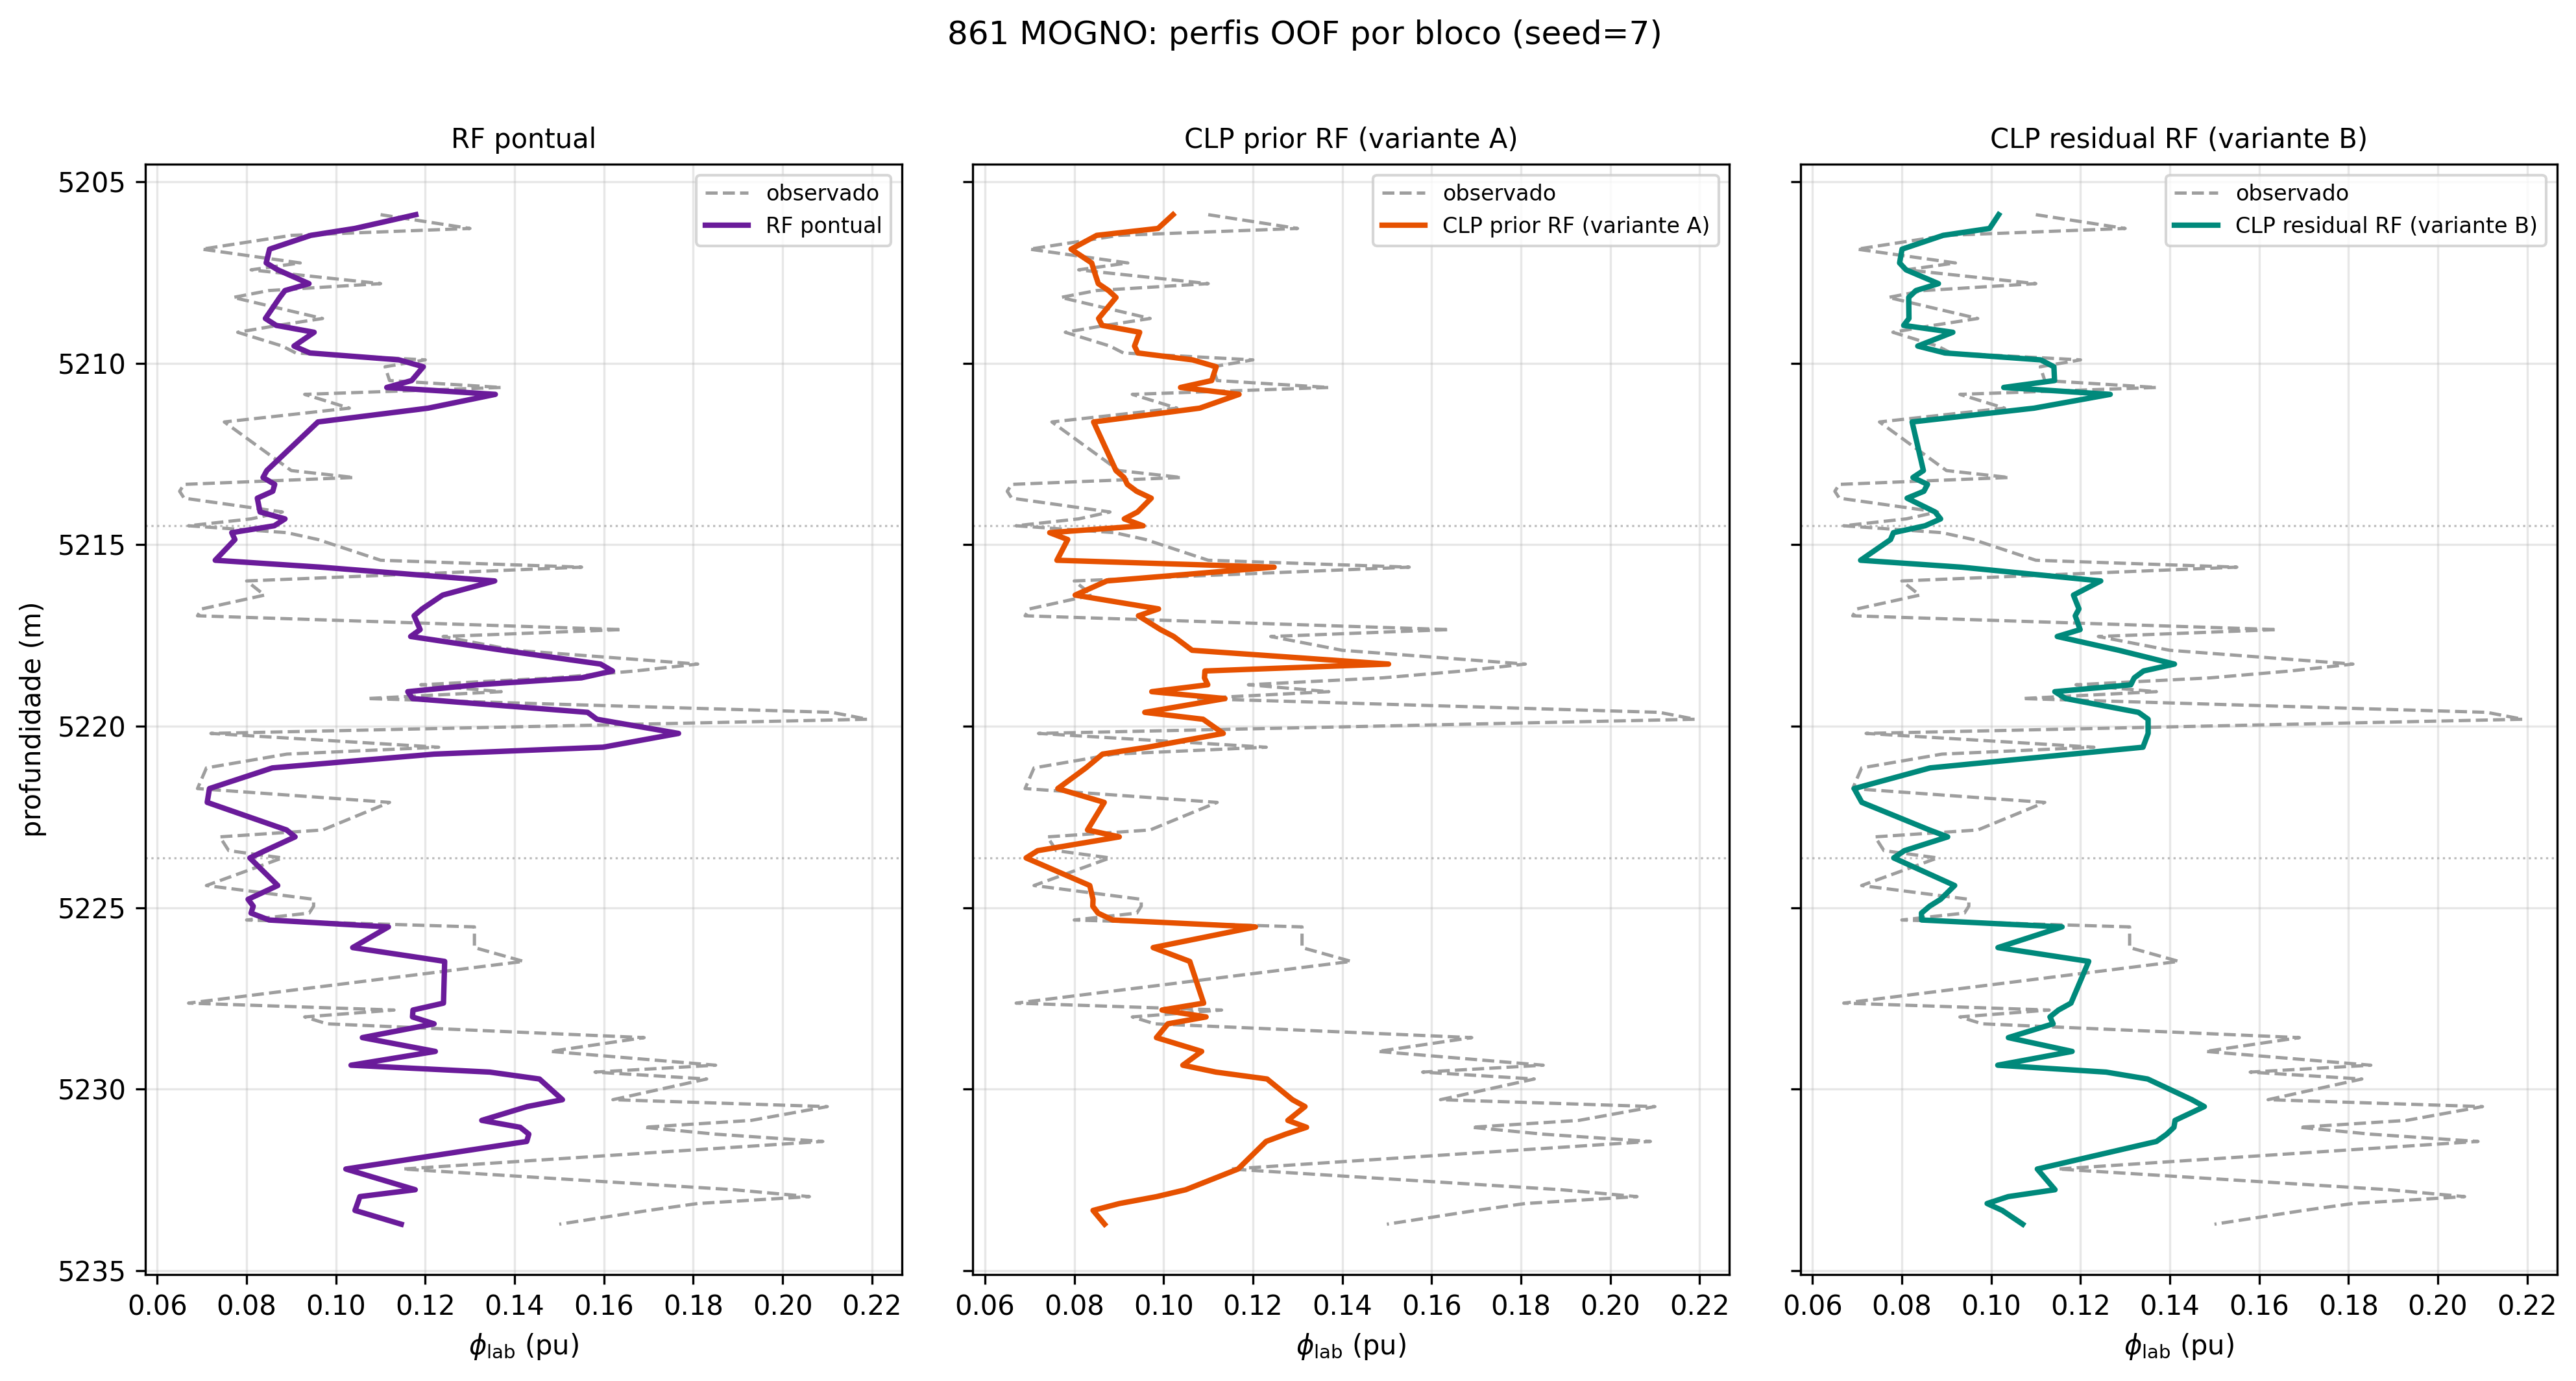
\includegraphics[width=\linewidth]{figures/fig_clp_three_methods_depth_panels.png}
  \caption{Perfis OOF de \philab{} ao longo da profundidade (\emph{seed}~7):
           observado (tracejado) versus RF pontual, CLP prior RF
           (variante~A) e CLP residual RF (variante~B), em painéis lado a
           lado. Linhas horizontais pontilhadas: limites entre blocos de
           teste.}
  \label{fig:clp_three_methods_depth}
\end{figure}

\begin{figure}[H]
  \centering
  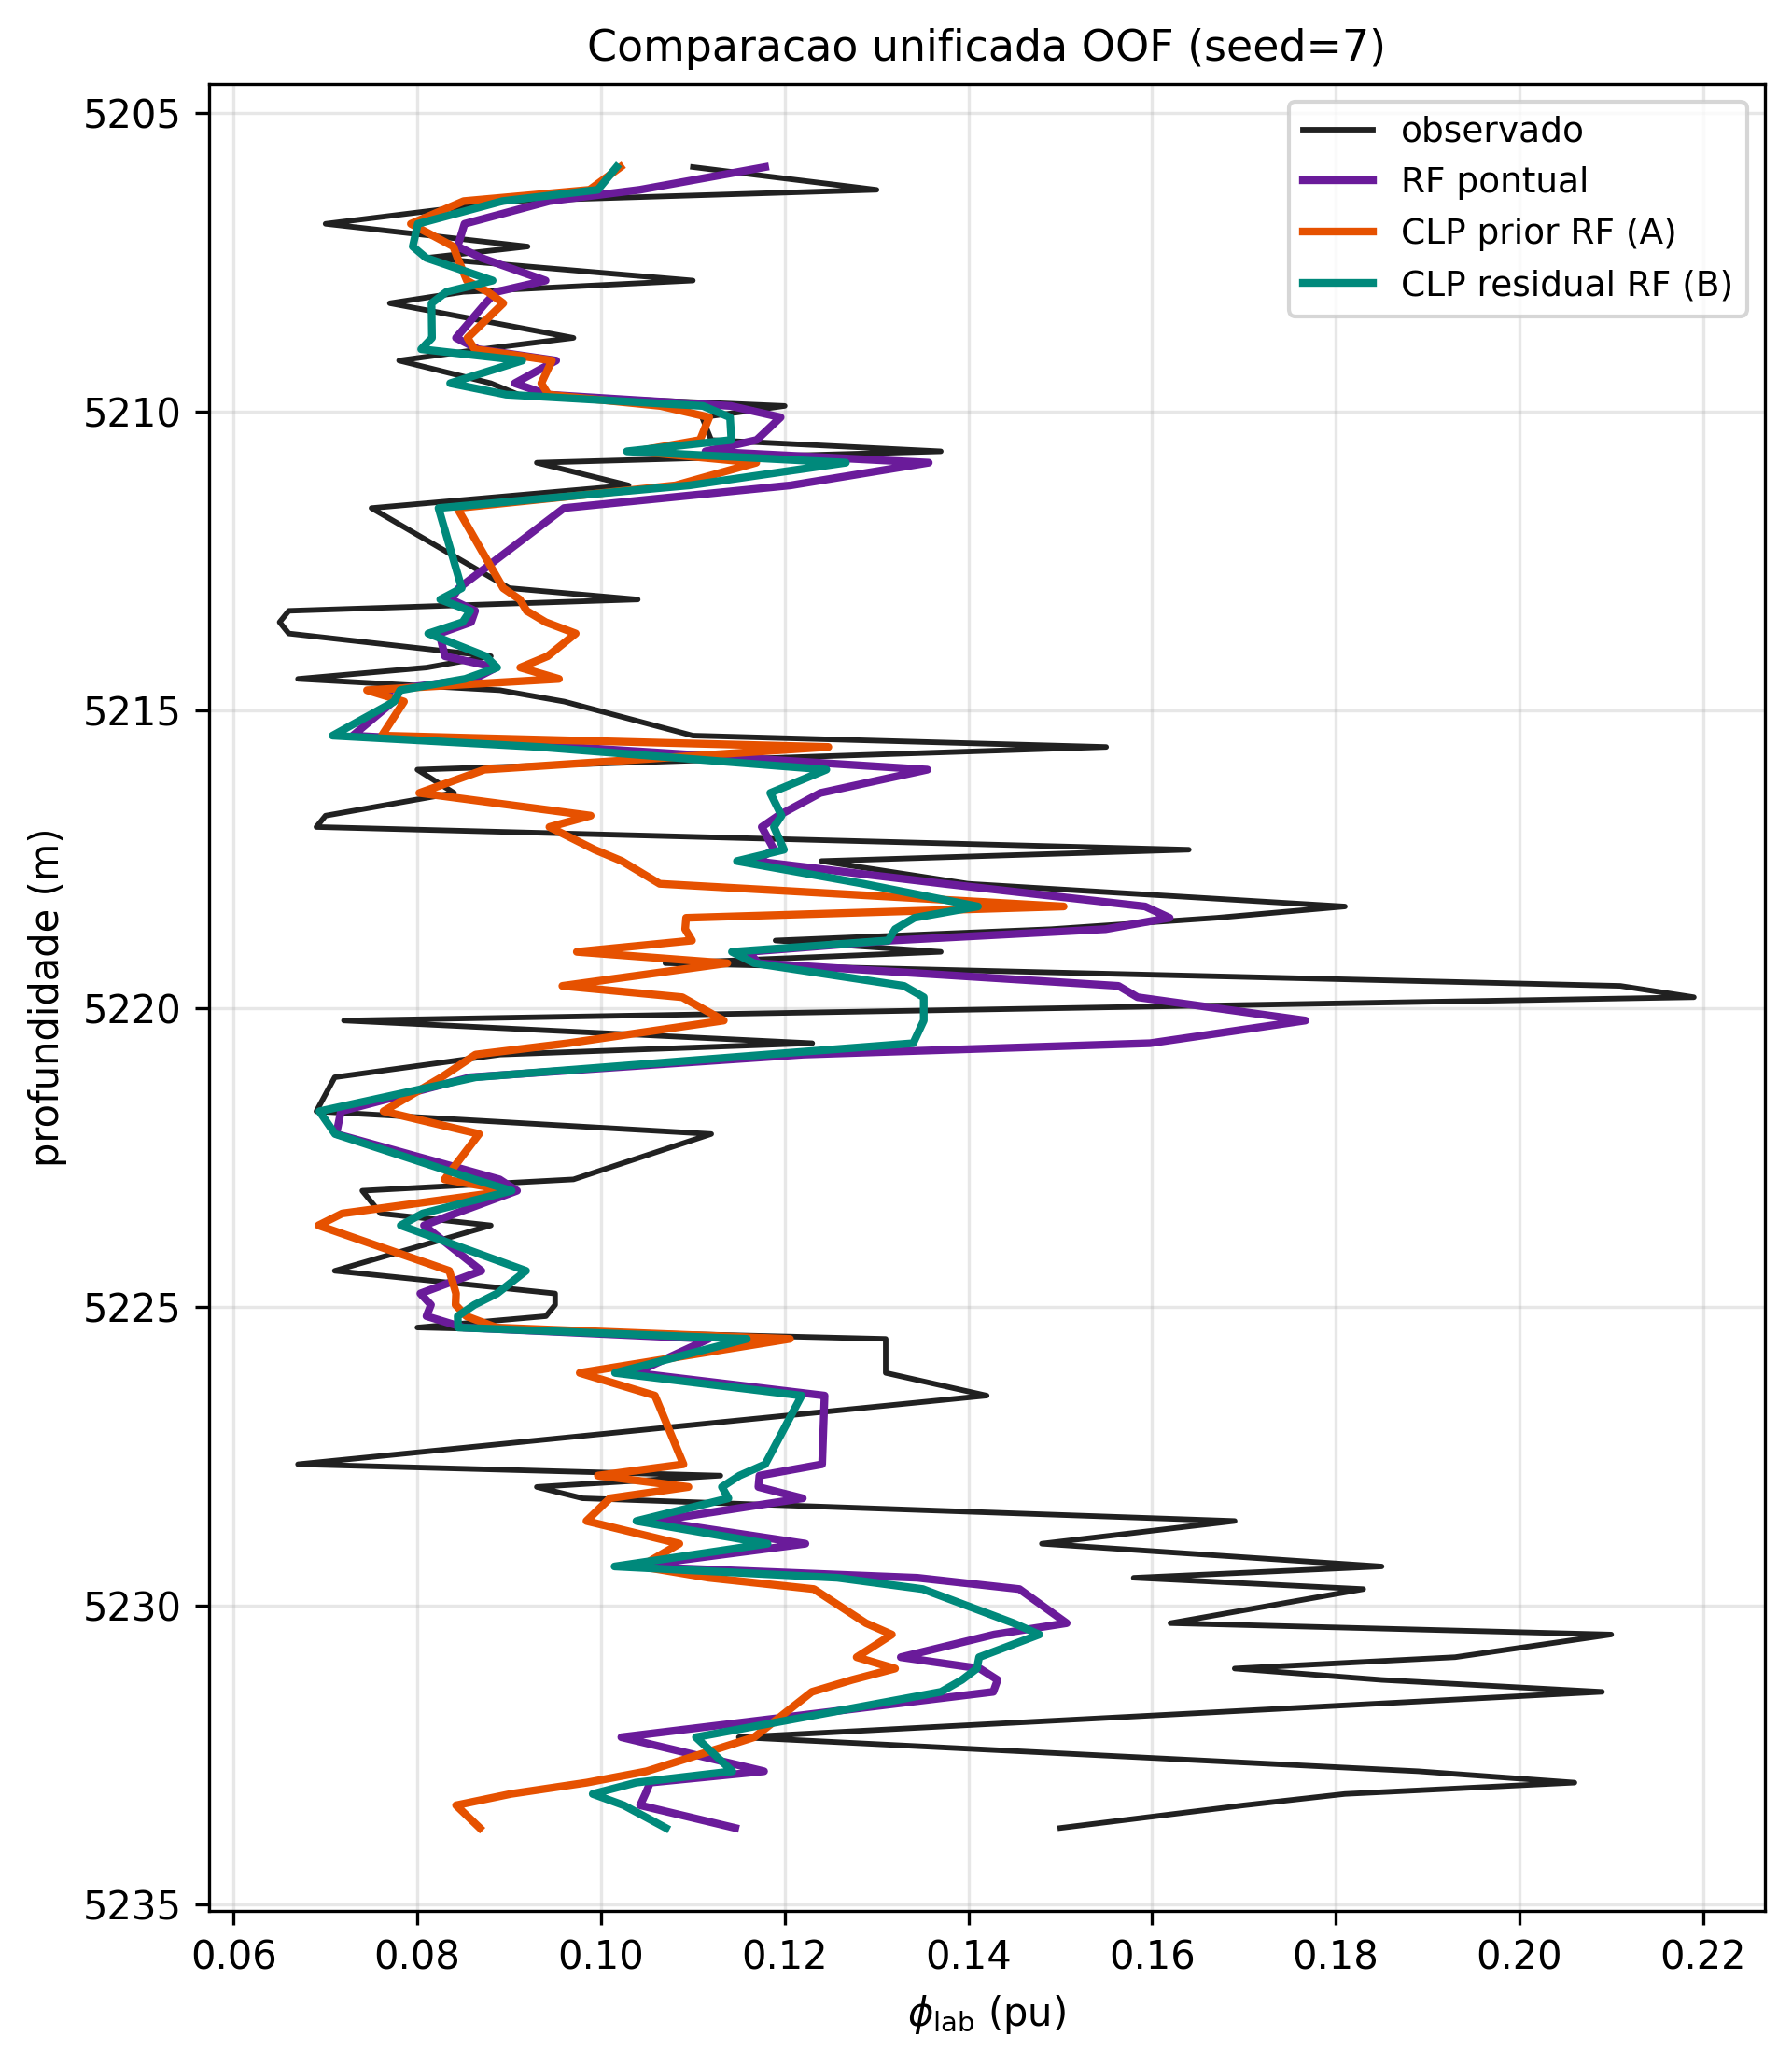
\includegraphics[width=0.62\linewidth]{figures/fig_clp_three_methods_depth_overlay.png}
  \caption{Mesmas curvas da Figura~\ref{fig:clp_three_methods_depth} em
           painel único: comparação direta das três predições OOF.}
  \label{fig:clp_three_methods_overlay}
\end{figure}

\subsection{Limitação visual e fidelidade à \philab{} observada}
\label{sec:clp_fidelity}

As Tabelas~\ref{tab:clp_vs_rf_global} e~\ref{tab:clp_vs_rf_blocks} medem
erro agregado (RMSE, $R^2$); a
Figura~\ref{fig:clp_three_methods_overlay} expõe um limite complementar:
\textbf{nenhuma} das três predições reproduz a \emph{morfologia fina} da
curva de \philab{} observada ao longo de todo o intervalo.
As curvas RF e CLP são visivelmente mais \emph{suaves} que o observado
(tracejado): picos e vales de laboratório (amplitude até $\approx 0{,}22$~pu
e quedas abaixo de $0{,}08$~pu) são atenuados pelas reconstruções, que
permanecem em faixa estreita ($\approx 0{,}08$--$0{,}16$~pu na maior
parte do poço).

A Tabela~\ref{tab:clp_fidelity} quantifica esse descompasso (\emph{seed}~7,
87 profundidades OOF).
A razão $\sigma_{\mathrm{pred}}/\sigma_{\mathrm{obs}}$ mede quanto da
variabilidade de \philab{} cada método preserva: valores bem abaixo de~1
indicam \emph{compressão} da amplitude.
A correlação de Pearson $r$ resume o alinhamento global; a coluna
$r(\Delta)$ correlaciona \emph{variações sucessivas} ao longo da
profundidade---proxy da capacidade de reproduzir oscilações locais entre
amostras adjacentes.

\begin{table}[H]
  \centering
  \caption{Fidelidade da curva OOF à \philab{} observada (\emph{seed}~7,
           $n=87$). $\sigma_{\mathrm{obs}}=0{,}043$~pu.}
  \label{tab:clp_fidelity}
  \small
  \begin{tabular}{lrrrr}
    \toprule
    Método & $\sigma_{\mathrm{pred}}/\sigma_{\mathrm{obs}}$ &
    $r$ & $r(\Delta)$ & MAE (pu) \\
    \midrule
    RF pontual & 0,59 & 0,58 & 0,09 & 0,027 \\
    CLP prior RF (A) & 0,37 & 0,59 & 0,10 & 0,029 \\
    CLP residual RF (B) & 0,50 & 0,63 & 0,13 & 0,027 \\
  \end{tabular}
\end{table}

\begin{table}[H]
  \centering
  \caption{RMSE OOF nas oito profundidades-plug versus demais amostras
           (\emph{seed}~7).}
  \label{tab:clp_plug_vs_nonplug}
  \begin{tabular}{lrr}
    \toprule
    Método & RMSE nos plugs (pu) & RMSE fora dos plugs (pu) \\
    \midrule
    RF pontual & 0,026 & 0,036 \\
    CLP prior RF (A) & \textbf{0,016} & 0,042 \\
    CLP residual RF (B) & 0,027 & 0,037 \\
    \bottomrule
  \end{tabular}
\end{table}

Na Tabela~\ref{tab:clp_fidelity}, as três abordagens capturam menos de
60\% do desvio padrão observado; a variante~A comprime ainda mais
($\sigma_{\mathrm{pred}}/\sigma_{\mathrm{obs}}\approx 0{,}37$), coerente
com a suavização adicional do AE em $\phi$ absoluta.
Os valores de $r(\Delta)\approx 0{,}09$--$0{,}13$ confirmam que nem RF nem
CLP acompanham a \emph{alta frequência} da série de laboratório de
amostra em amostra---apenas a tendência de baixa frequência visível na
Figura~\ref{fig:clp_three_methods_overlay}.

A Tabela~\ref{tab:clp_plug_vs_nonplug} explica por que a variante~A
piora globalmente apesar de parecer próxima do observado em alguns trechos:
nas oito profundidades com plug na máscara fixa, o RMSE da~A
($0{,}016$~pu) é o menor dos três; \emph{fora} dos plugs, porém, sobe para
$0{,}042$~pu---pior que o RF ($0{,}036$~pu).
O CLP absoluto ajusta melhor localmente onde há amarra, mas distorce o
intervalo entre plugs.
A variante~B mantém RMSE fora dos plugs ($0{,}037$~pu) próximo ao RF e
só oferece refinamento modesto nos plugs.

\paragraph{Por que as curvas ``não conversam'' com o observado.}
Quatro mecanismos se somam, além do limite informacional do wireline já
discutido na Seção~\ref{sec:discussao} (Tabela~\ref{tab:corr_phi}):
\begin{enumerate}
  \item \textbf{Escala de informação.} Correlações fortes entre porosidades
        de perfil e \philab{} ($r\approx 0{,}7$) não implicam reprodução
        ponto a ponto: o perfil integra um volume lateral distinto do
        testemunho de laboratório, com heterogeneidade subescala que as
        oito curvas wireline não resolvem.
  \item \textbf{Suavização estrutural.} O AE em janelas de $L=16$, o
        \emph{stitching} por média e o termo $\lambda\|z-z_0\|^2$ impõem
        curvas latentes regulares; o inverso não interpola \philab{} exata
        em cada profundidade, e sim uma reconstrução acoplada ao longo da
        janela (Seção~\ref{sec:clp_balance}).
  \item \textbf{Esparsidade das amarras.} Dez plugs em 87 amostras
        deixam a maior parte das janelas com $m=0$; o laboratório altera
        o perfil apenas onde janelas com plug passam, sem fixar cada
        amostra.
  \item \textbf{Validação honesta.} Na validação por blocos, o bloco de
        teste não entra no treino; no bloco~2 (Tabela~\ref{tab:clp_vs_rf_blocks})
        todos os métodos degradam, pois o wireline responde de forma
        distinta no intervalo mais permeável.
\end{enumerate}

\paragraph{Leitura para o produto petrofísico.}
Se o critério de sucesso for \emph{replicar visualmente} a curva de
\philab{} em todas as 87 amostras, os resultados da Etapa~1f são
\textbf{insatisfatórios} em todos os casos---incluindo a variante~B, que
só empata o RF em RMSE global sem ganho visual decisivo.
Se o critério for \emph{estimar tendência de porosidade} condicionada ao
perfil (e fracamente ao lab nos plugs), o RF e a variante~B permanecem
\emph{marginalmente aceitáveis} como insumo preliminar para a Etapa~2,
com a mesma ressalva do bloco inferior já documentada na
Seção~\ref{sec:wellprofile}.
O CLP deve ser interpretado como experimento de formulação inversa sem
vazamento, não como substituto operacional da curva de laboratório.

\subsection{Estudo de sensibilidade e teto informacional}
\label{sec:clp_sensitivity}

Para verificar se a baixa fidelidade visual
(Seção~\ref{sec:clp_fidelity}) poderia ser corrigida por ajuste de
hiperparâmetros do autoencoder ou do otimizador latente, executamos um
estudo complementar com \emph{seed}~7 e o mesmo protocolo de blocos:
(i)~baselines de teto informacional e interpolação mecânica;
(ii)~ablação \emph{one-factor-at-a-time} (OFAT) na variante~B
(CLP residual), variando um parâmetro por vez em relação ao
default ($L=16$, latente $=16$, oculto $=128$, 200 épocas AE,
lr$_{\mathrm{opt}}=0{,}05$).

\begin{table}[H]
  \centering
  \caption{Baselines e teto informacional para \philab{} ($n=87$,
           \emph{seed}~7). $\phi_{ND}$ e \phiN{}: curva de perfil
           usada diretamente (sem ML).}
  \label{tab:clp_sensitivity_baselines}
  \small
  \begin{tabular}{llrrrr}
    \toprule
    Caso & Tipo & RMSE (pu) & $R^2$ & $\sigma$ ratio & $r(\Delta)$ \\
    \midrule
    $\phi_{ND}$ perfil & wireline & 0,032 & 0,446 & 0,87 & 0,27 \\
    \phiN{} perfil & wireline & 0,039 & 0,164 & 0,98 & 0,27 \\
    RF pontual OOF & ML & 0,036 & 0,304 & 0,59 & 0,09 \\
    Spline linear nos plugs & mecânico & 0,090 & $-3{,}49$ & 2,07 & $-0{,}08$ \\
    CLP residual (default) & CLP-B & 0,036 & 0,290 & 0,50 & 0,13 \\
    \bottomrule
  \end{tabular}
\end{table}

\begin{table}[H]
  \centering
  \caption{Ablação OFAT na variante~B (CLP residual): $\Delta$RMSE em
           relação ao default (pu). Nenhuma variação altera
           $\sigma_{\mathrm{pred}}/\sigma_{\mathrm{obs}}$ de forma
           relevante (faixa 0,49--0,50 em todos os casos).}
  \label{tab:clp_sensitivity_ofat}
  \small
  \begin{tabular}{llrr}
    \toprule
    Fator variado & Valores testados & $\Delta$RMSE (pu) \\
    \midrule
    Dimensão latente & 8, 32 & $0{,}000$, $-0{,}0001$ \\
    Camada oculta AE & 64, 256 & $0{,}000$, $0{,}000$ \\
    Épocas AE & 100, 400 & $-0{,}000$, $-0{,}000$ \\
    lr otimizador $z$ & 0,01, 0,10 & $0{,}000$, $0{,}000$ \\
    Comprimento janela $L$ & 8, 24 & $-0{,}0004$, $-0{,}000$ \\
    \bottomrule
  \end{tabular}
\end{table}

Na Tabela~\ref{tab:clp_sensitivity_baselines}, o uso direto de $\phi_{ND}$
do perfil atinge o menor RMSE (0,032~pu) e a maior razão de variância
preservada ($\sigma$ ratio $=0{,}87$), porém \emph{ainda abaixo de~1}:
nem o melhor log de perfil reproduz toda a variabilidade da
\philab{}.
A porosidade de nêutron fica próxima em amplitude ($\sigma$ ratio
$\approx 0{,}98$), mas com RMSE maior.
O RF OOF e o CLP default ficam em $\sigma$ ratio $\approx 0{,}59$ e
$0{,}50$, respectivamente---confirmando a leitura visual da
Figura~\ref{fig:clp_three_methods_overlay}.
A interpolação linear OOF entre os plugs de treino por bloco falha
fortemente (RMSE $=0{,}090$~pu, $R^2\ll 0$): poucas amarras não sustentam
uma curva de laboratório entre blocos sem informação de perfil.

A Tabela~\ref{tab:clp_sensitivity_ofat} mostra que alterar profundidade
efetiva da rede, taxa de aprendizado do inverso, épocas do AE ou
comprimento de janela ($L=8$--24) desloca o RMSE global em no máximo
$0{,}0004$~pu e \emph{não} eleva $\sigma$ ratio para a faixa do
observado.
A melhor janela curta ($L=8$) melhora marginalmente RMSE e $r(\Delta)$,
mas mantém $\sigma$ ratio $\approx 0{,}50$: captura um pouco mais de
variação local, porém longe de reproduzir os picos da curva preta.
Na seleção interna de $\lambda$ por fold, o valor escolhido ficou no
\emph{mínimo} da grade ($0{,}0001$) na variante~B---ou seja, o modelo
já preferia confiar mais no termo de dados do que no prior latente;
a baixa fidelidade de alta frequência não é explicada por
super-regularização.

\paragraph{Conclusão do estudo de sensibilidade.}
Os resultados apoiam a hipótese de \textbf{limite informacional e
estrutural} (wireline + poucos plugs + suavização do AE/stitching), e
\textbf{não} de hiperparâmetro mal ajustado: mesmo $\phi_{ND}$ direto
---upper bound simples do perfil--- não atinge $\sigma$ ratio $=1$;
a ablação OFAT do CLP-B é estável em RMSE e em amplitude.
Investimento adicional em \emph{tuning} de rede ou otimizador, neste
poço e protocolo, tem retorno esperado baixo frente a usar $\phi_{ND}$
ou RF como tendência e reservar \philab{} para calibração pontual.

\subsection{Síntese da Etapa~1f}

O experimento confirma que \emph{ter} laboratório esparso nos plugs não
garante superar o RF pontual se a formulação reconstrói $\phi$ absoluta:
a variante A fica claramente abaixo do baseline.
A reparametrização residual preserva o RF onde não há amarra e delega ao
CSGM apenas correções locais---comportamento alinhado à física do
problema (wireline domina a escala global; laboratório calibra pontos).
Ainda assim, no poço~861, o ganho global da variante B é marginal e não
altera a recomendação principal da Etapa~1: usar RF ou \phiND{} como
insumo de porosidade para a Etapa~2.
A Seção~\ref{sec:clp_fidelity} mostra que, além das métricas agregadas,
as curvas recuperadas \emph{não reproduzem} a variabilidade fina da
\philab{} observada---limitação estrutural e informacional, não falha de
implementação isolada.
O estudo de sensibilidade (Seção~\ref{sec:clp_sensitivity}) confirma essa
leitura com baselines de teto ($\phi_{ND}$, spline nos plugs) e ablação
OFAT de hiperparâmetros.
O CLP residual permanece documentado como alternativa metodológica quando
se deseja fundir perfil e amarras de laboratório sem vazamento, com
expectativa realista de refinamento local e não de substituição do RF em
todo o intervalo nem de réplica visual da curva de laboratório.

\section{Discussão}
\label{sec:discussao}

Esta seção sintetiza os achados das tabelas e figuras anteriores
sob três eixos: limite de informação do perfil, papel da validação
geológica e encaminhamento para a modelagem física de velocidades.

\subsection{O problema é a informação, não o algoritmo}

Os resultados negativos para FZI e permeabilidade não indicam erro no
pipeline de dados ou nos scripts.
O teste \emph{oracle} (Figura~\ref{fig:oracle}) mostra que o FZI \emph{tem}
sinal previsível quando porosidade e permeabilidade de laboratório
estão disponíveis (Tabela~\ref{tab:corr_fzi})---mas essas variáveis
são justamente excluídas do modelo para que ele aprenda apenas do perfil.

Trocar RF por rede neural, GAM ou regressão linear não muda essa
conclusão para FZI (Tabela~\ref{tab:regressors}).
Para porosidade, o RF permaneceu o melhor entre regressores pontuais
(Tabela~\ref{tab:phi_models}), embora o ganho seja modesto ($R^2 \approx
0{,}15$).
O CLP-CSGM com laboratório esparso (Seção~\ref{sec:clp}) não superou o
RF na formulação absoluta com prior RF; a variante residual quase empata
globalmente e melhora localmente no bloco superior, mas não altera o
papel do RF como estimativa principal ao longo do poço.
O estudo de sensibilidade da Seção~\ref{sec:clp_sensitivity} indica que
ajuste fino de arquitetura ou otimizador do CLP não recupera a
variabilidade fina da \philab{}; o teto informacional do perfil
($\phi_{ND}$ direto) também permanece abaixo da variância observada.

\subsection{Porosidade: único resultado utilizável}
\label{sec:discussao_phi}

O encadeamento diagnóstico $\rightarrow$ regressão confirma coerência
interna dos resultados.
A Tabela~\ref{tab:corr_phi} mostra correlações fortes ($r > 0{,}67$)
entre porosidades de perfil e \philab{}; a Tabela~\ref{tab:phi_folds}
mostra $R^2$ positivo nos blocos~0 e~1 e negativo no bloco~2.
Na prática, isso significa que o RF de porosidade pode ser usado como
\emph{estimativa preliminar} ao longo do poço, com ressalva explícita
para o intervalo 5225--5234~m, onde o modelo perde validade.
As Figuras~\ref{fig:clp_three_methods_overlay} e a
Tabela~\ref{tab:clp_fidelity} reforçam que nem RF nem CLP replicam a
morfologia fina da \philab{} observada---apenas tendência de baixa
frequência.
Uma alternativa conservadora é usar diretamente \phiND{} do perfil,
sem modelo de aprendizado de máquina, quando a simplicidade for preferível.

\subsection{FZI e permeabilidade: descartados como alvo de perfil}
\label{sec:discussao_fzi}

O FZI resume textura e qualidade de zona de fluxo---propriedades que o perfil
convencional não mede diretamente.
A Figura~\ref{fig:fzi_corr}, a Tabela~\ref{tab:corr_fzi} e o teste
\emph{oracle} (Figura~\ref{fig:oracle}) contam a mesma história: o perfil
não vê o que o laboratório vê.
A permeabilidade apresenta ainda maior dificuldade: distribuição com
cauda longa (bloco~2, Tabela~\ref{tab:depthblocks}) e $R^2$ fortemente
negativo em todos os algoritmos (Tabela~\ref{tab:regressors}).

\subsection{Por que a validação por blocos importa}

A validação por blocos de profundidade expõe mudanças litológicas
reais (Tabela~\ref{tab:depthblocks}).
No bloco~1, onde predomina \emph{Grainstone} (litotipo~1), o modelo de FZI colapsa
(Tabela~\ref{tab:fzi_folds}).
Métricas obtidas com divisão aleatória 80/20 devem ser vistas apenas
como referência histórica, não como prova de que o modelo funcionaria
em um intervalo novo do poço.

\subsection{Papel do microCT nesta fase}

Incluir descritores de microCT não melhorou o RF nos dez plugs
(Tabela~\ref{tab:ctplugs}).
Isso não diminui o valor do microCT para o projeto: na Etapa~2, a
geometria dos poros (razão de aspecto, fração de sólidos) servirá
para calibrar os modelos DEM/SC, e não como variável extra num
regressor de perfil.

\subsection{Caminho para $V_p/V_s$ (Etapa~2)}

A cadeia recomendada, em ordem, é:
\begin{enumerate}
  \item Estimar porosidade a partir do perfil (\philab{} via RF ou
        \phiND{} diretamente).
  \item Segmentar o intervalo por HFU (preferir HFU de laboratório;
        a predição por logística da Tabela~\ref{tab:hfu_class} é
        apenas um recurso auxiliar).
  \item Usar geometria de poros dos dez plugs CT para parametrizar DEM/SC.
  \item Calcular $V_p$ e $V_s$ teóricos por HFU no Pyrockphys.
  \item Só então considerar aprendizado de máquina sobre resíduos
        (Etapa~3), após validar a modelagem física.
\end{enumerate}

\section{Conclusões e recomendações}
\label{sec:conclusoes}

\begin{enumerate}
  \item \textbf{Porosidade:} manter RF (ou \phiND{} do perfil) como
        insumo para DEM/SC. O $R^2 \approx 0{,}15$ é modesto, mas é o
        único resultado regressivo estável no perfil completo. O CLP
        residual sobre RF (Etapa~1f) quase reproduz esse patamar, porém
        sem ganho global decisivo; usar apenas se amarras esparsas de
        laboratório forem obrigatórias na entrega de curva.
  \item \textbf{FZI:} não usar previsão direta a partir de perfis como
        produto final. O perfil não carrega informação suficiente.
  \item \textbf{HFU:} priorizar classificação de laboratório;
        a predição automática (36\% de acurácia) serve apenas como
        recurso auxiliar (\emph{fallback}).
  \item \textbf{microCT:} avançar para Etapa~2, usando os dez plugs para
        calibrar geometria de poros nos modelos DEM/SC.
  \item \textbf{Ajuste de modelos:} adiar busca fina de hiperparâmetros
        até definir claramente os insumos da modelagem física.
  \item \textbf{Motivação para a Etapa~2:} o limite não é apenas
        algoritmico---é de \textbf{informação nas curvas de perfil}
        para FZI, permeabilidade e velocidades. Isso justifica investir em
        física de rochas (DEM/SC + microCT + HFU de laboratório), não em
        mais \emph{tuning} de ML perfil $\rightarrow$ $V_p$.
\end{enumerate}

\section*{Disponibilidade dos dados e reprodutibilidade}

A integração de perfis, laboratório e microCT, bem como os
protocolos de validação, treinamento e diagnóstico descritos neste
relatório, foram implementados de forma automatizada e reprodutível.
Os conjuntos processados, métricas numéricas e figuras podem ser
obtidos mediante solicitação aos autores ou acesso ao repositório
do projeto de pesquisa.

Os experimentos CLP da Seção~\ref{sec:clp} usam máscara fixa nos dez
plugs, validação por três blocos de profundidade e comparação OOF
alinhada ao RF pontual; as tabelas reportadas referem-se à \emph{seed}~7
(junho de 2026).
Os valores numéricos e figuras comparativas podem ser reproduzidos a
partir dos artefatos tabulares do repositório do projeto, mediante
solicitação aos autores.
O estudo de sensibilidade da Seção~\ref{sec:clp_sensitivity} (baselines,
ablação OFAT da variante~B) pode ser repetido com o orquestrador
dedicado de sensibilidade da Etapa~1f (\emph{seed}~7).

\end{document}
